%% Control Engineering Practice submission manuscript.
%% Template source: Elsevier elsarticle bundle (numbered-reference example,
%% downloaded from the official Elsevier LaTeX instructions on 18 Aug. 2026).
\documentclass[final,5p,twocolumn]{elsarticle}
\usepackage{fontspec}
\usepackage{xeCJK}
\setmainfont{TeX Gyre Termes}
\setCJKmainfont[AutoFakeBold=2,AutoFakeSlant=0.2]{Noto Serif CJK SC}
\setCJKsansfont{Noto Sans CJK SC}
\setCJKmonofont{Noto Sans Mono CJK SC}
\usepackage{amsmath,amsfonts,amssymb,bm}
\usepackage{mathtools}
\usepackage{xcolor}
\usepackage{algorithmic}
\usepackage{algorithm}
\renewcommand{\algorithmicrequire}{\textbf{输入：}}
\renewcommand{\algorithmicensure}{\textbf{保证：}}
\renewcommand{\algorithmicif}{\textbf{若}}
\renewcommand{\algorithmicthen}{\textbf{则}}
\renewcommand{\algorithmicelse}{\textbf{否则}}
\renewcommand{\algorithmicelsif}{\textbf{否则若}}
\renewcommand{\algorithmicfor}{\textbf{循环}}
\renewcommand{\algorithmicdo}{\textbf{执行}}
\renewcommand{\algorithmicend}{\textbf{结束}}
\renewcommand{\algorithmicreturn}{\textbf{返回}}
\usepackage{array}
\allowdisplaybreaks
\usepackage{subfig}
\captionsetup[subfloat]{font=small,labelfont=normalfont,
  justification=centering,singlelinecheck=true}
\captionsetup{skip=4pt}
\usepackage{textcomp}
\usepackage{url}
\usepackage{verbatim}
\usepackage{booktabs}
\usepackage{graphicx}
\usepackage{float}
\usepackage{placeins}
\usepackage{multirow}
\abstracttitle{摘要}
\keywordtitle{关键词}
\renewcommand{\figurename}{图}
\renewcommand{\tablename}{表}
\renewcommand{\refname}{参考文献}
\renewcommand{\appendixname}{附录}
\floatname{algorithm}{算法}
\myfooter[L]{投稿至 \emph{Control Engineering Practice} 的中文译稿\hfill 2026年8月28日}
% Permit compact, ordered float packing in the two-column review layout.
\setcounter{topnumber}{4}
\setcounter{bottomnumber}{2}
\setcounter{totalnumber}{6}
\setcounter{dbltopnumber}{2}
\renewcommand{\topfraction}{0.95}
\renewcommand{\bottomfraction}{0.80}
\renewcommand{\textfraction}{0.05}
\renewcommand{\floatpagefraction}{0.88}
\renewcommand{\dbltopfraction}{0.95}
\renewcommand{\dblfloatpagefraction}{0.88}
\setlength{\textfloatsep}{6pt plus 2pt minus 2pt}
\setlength{\floatsep}{5pt plus 2pt minus 2pt}
\setlength{\intextsep}{5pt plus 2pt minus 2pt}
\setlength{\dbltextfloatsep}{6pt plus 2pt minus 2pt}
\setlength{\dblfloatsep}{5pt plus 2pt minus 2pt}
% Elsevier Editorial Manager does not preserve source subdirectories, so the
% submission artwork is kept beside this file in CEP/.
\graphicspath{{./}}
\hyphenation{au-ton-o-mous over-taking race-car}
% Ignore only sub-2-pt class-rounding noise; substantive boxes are fixed below.
\hfuzz=1.95pt

% --- Math shortcuts ---
\newcommand{\R}{\mathbb{R}}
\newcommand{\E}{\mathbb{E}}
\newcommand{\norm}[1]{\left\lVert#1\right\rVert}
\newcommand{\diag}{\operatorname{diag}}
\DeclareMathOperator*{\argmin}{arg\,min}
\DeclareMathOperator*{\argmax}{arg\,max}
\newcommand{\IEEEPARstart}[2]{#1#2}
\newcommand{\IEEEmembership}[1]{#1}

\journal{Control Engineering Practice}

\begin{document}

\begin{frontmatter}

\title{面向自动驾驶赛车超车的博弈引导战术走廊学习}

\author[bit]{Shuyi Gao}
\author[bit]{Ren Jin}
\author[bit]{Defu Lin}
% AUTHOR_INPUT_NEEDED: designate the corresponding author and add \ead{...}.

\affiliation[bit]{organization={北京理工大学宇航学院},
                  city={北京},
                  country={中国}}

\begin{abstract}
交互式超车不仅要求选择超车侧：战术决策还必须在对手响应过程中保持一致，
并为下游规划器留出足够的执行空间。直接博弈求解能够刻画交互，但在线计算代价高；
离散机动标签和单条轨迹无法为规划器提供持续约束；端到端策略则难以显式判断决策是否可执行。
本文提出一种博弈引导的战术走廊策略，将时变可行集而非执行器指令作为学习决策变量。
鲁棒 Stackelberg 响应集教师为截断分位数评论家（TQC）提供响应集最优动作先验和动作条件
鲁棒价值标签，将离线交互推理摊销为一次策略评估。策略输出请求速度上限、超车侧承诺和
Frenet 走廊。具有优先级的状态机和确定性裁剪器保持所选侧并剔除坍缩区间；候选动作在发布前
经过保守的参考层轮胎需求筛选。受走廊约束的序列二阶锥规划、速度剖面生成器以及参考条件
轮廓误差非线性模型预测控制器进一步生成油门、制动、转向和挡位指令。该方法在硬件在环平台
上进行验证：完整算法运行于目标 Neousys RGS-8805GC 计算机，并通过两路控制器局域网（CAN）
与独立服务器上的 EAV24 模拟器通信。被控对象包含动力总成、制动、转向、悬架、空气动力、
热轮胎和传感器等子系统动力学。在1000圈闭环评估中，完整方法取得94.7\%的超车成功率
（95\%精确二项置信区间为93.1--96.0\%），且未观察到碰撞或越出赛道边界。配对比较和组件
消融表明，性能提升主要来自学习式走廊塑形、博弈引导和持续的侧向承诺。现有证据限于由
模拟器提供车辆状态和对手信息的双车交互。
\end{abstract}

\begin{keyword}
自动驾驶赛车 \sep 博弈引导强化学习 \sep 战术走廊
\sep 交互式超车 \sep 硬件在环仿真
\end{keyword}

\end{frontmatter}

% =====================================================================
\section{引言}
% =====================================================================
自动驾驶赛车使控制系统处于战术交互与轮胎力极限在相近时间尺度上共同演化的工况。
后车必须在可用空间闭合之前选择超车机会，但只有当下游规划器能够构造连续路径、控制器能够
通过物理执行器接口实现该路径时，这一决策才具有实际意义。阿布扎比自动驾驶赛车联赛
（A2RL）等全尺寸赛事使这种耦合具有直接工程意义：赛车软件运行于车载硬件，持续观测其他
非合作车辆，并必须在严格实时回路中输出线控指令~\cite{betz2022survey,hoffmann2026a2rl}。
因此，核心控制问题不只是避碰或底层跟踪，而是如何将面向对手的战术推理转化为一种在反复
重规划过程中仍具有明确几何含义、时间持续性和可执行性的超车机会。

\subsection{相关工作}

传统超车规划器通过分层机动选择或显式动态博弈组织交互。分层架构将跟随、防守或超车决策
与下游路径和速度生成分离，具体方法涵盖有限状态超车分解和滚动时域赛车规划器
~\cite{sureshbabu2022autopass,kim2023hierarchical,jung2023iac,
thakkar2024hierarchical,toschi2025modular,hoffmann2026a2rl}。博弈论方法则利用
Stackelberg、贝叶斯、约束势博弈或近势博弈形式耦合竞争车辆的目标，使自车能够预判封堵和
反制机动~\cite{ji2023hierarchicalgame,jia2023bayesian,kalaria2025alpha,
lopez2022payoff,swain2023cooperative}。这些方法显式描述战略角色和预测响应，但在线优化通常
在每次更新中将交互归结为一个选定响应和一个局部最优机动。

学习方法将交互式决策摊销为固定代价的策略评估。深度强化学习已展现出具有竞争力的赛车性能，
博弈信息、轨迹辅助和图结构策略进一步把学习决策扩展到对手交互与超车
~\cite{wurman2022gtsophy,yuan2022drlgame,lin2023limit,
evans2023trajectory,hell2024lidar,hu2023dynamicgraph,
baumann2025predictive,han2024marl}。近期混合方法将学习式战术引导与结构化预测或优化相结合：
深度强化学习可主动塑造换道交互、协调汇入顺序并引导多车走廊
~\cite{liu2023proactive,muzahid2025merging,yang2026corridor}；人类引导的策略更新还可提升
学习驾驶策略的稳定性~\cite{guo2025rlhf}。这类方法能够提供快速在线决策和丰富交互特征，
同时在需要显式轨迹约束时保留基于模型的规划。

上述两类研究仍留下一个具体的规划接口问题：博弈求解器虽能给出对手响应，却反复将其收缩为
单个在线解；学习策略则很少把超车侧承诺保留为规划器可直接使用的显式可行域。本文采用鲁棒
Stackelberg 响应集教师同时监督投影后的战术动作及其动作条件价值，以解决这一衔接问题。
TQC 将该监督蒸馏为一次策略评估，确定性混合逻辑再把决策发布为持续锁定侧向的 Frenet 走廊
和速度请求。由此，战略交互能够进入滚动时域规划，而不会将战术输出简化为机动标签或单条
参考轨迹。

\subsection{主要贡献与文章结构}

本文面向交互式超车提出一种博弈监督的战术走廊策略。鲁棒 Stackelberg 响应集教师根据一组
近最优对手响应评估投影后的战术候选；TQC 蒸馏相应的动作先验和动作条件鲁棒价值；确定性混合
逻辑则将策略样本转化为持续且可审计的规划器边界。固定的下游执行器用于检验学习可行集能否
在闭环中实现。

本文的主要贡献如下：
\begin{enumerate}
    \item 将战术超车表述为鲁棒可行集选择问题，并构造 Stackelberg 响应集教师，以传递响应集
    最优投影动作和动作条件鲁棒价值标签。后者通过仅在训练阶段使用的辅助头监督共享的分布式
    评论家编码器，同时 TQC 抑制由罕见高回报超车序列引起的乐观更新。

    \item 提出一种与规划器兼容的混合接口，将学习得到的时变走廊与带滞回的侧向承诺、确定性
    对手足迹裁剪和参考层轮胎可接受性投影相结合。该接口抑制相邻更新间的侧向切换，拒绝几何
    坍缩走廊，并发布可独立于学习策略检查的横向边界和速度上限。

    \item 在目标硬件在环回路中评估战术方法。完整算法栈运行于 A2RL RGS-8805GC 计算机，
    通过两路 CAN 与 EAV24 被控对象交换车辆、对手、赛事控制和四通道执行器数据。配对基线
    与消融实验检验战术有效性、组件必要性和闭环失效模式。
\end{enumerate}

第~\ref{sec:model}节介绍车辆、轮胎包络和赛道模型；第~\ref{sec:tactical}节给出博弈引导
走廊策略；第~\ref{sec:execution}节概述通用的走廊约束参考生成与闭环跟踪层；
第~\ref{sec:experiments}节报告硬件在环评估；第~\ref{sec:discussion}节讨论证据及其局限性。

% =====================================================================
\begingroup
\setlength{\abovedisplayskip}{6pt plus 1pt minus 1pt}
\setlength{\belowdisplayskip}{6pt plus 1pt minus 1pt}
\setlength{\abovedisplayshortskip}{4pt plus 1pt minus 1pt}
\setlength{\belowdisplayshortskip}{4pt plus 1pt minus 1pt}
\setlength{\jot}{2pt}
\section{车辆、轮胎与赛道模型}\label{sec:model}
% =====================================================================
考虑封闭赛道上的自车 $e$ 和非合作对手车 $o$。战术层与执行层采用平面车辆动力学、
随速度变化的轮胎加速度包络，以及交互关系与路径几何的 Frenet 表示。

对于车辆 $i\in\{e,o\}$，$X_i,Y_i$ 和 $\psi_i$ 分别表示惯性系位置与航向角，
$v_{x,i},v_{y,i}$ 和 $r_i$ 分别表示车体系速度与横摆角速度。车速和质心侧偏角为
$V_i=\sqrt{v_{x,i}^2+v_{y,i}^2}$，
$\beta_i=\operatorname{atan2}(v_{y,i},v_{x,i})$。令
$\mathcal W=\{\mathrm{fl},\mathrm{fr},\mathrm{rl},\mathrm{rr}\}$ 表示四个车轮，
$\bm r_q=[x_q,y_q]^\top$ 表示车轮 $q$ 相对于车辆质心的位置。平面四轮动力学为
\begin{equation}
\begin{bmatrix}
\dot X_i\\
\dot Y_i\\
\dot\psi_i\\
\dot v_{x,i}\\
\dot v_{y,i}\\
\dot r_i
\end{bmatrix}
=
\begin{bmatrix}
v_{x,i}\cos\psi_i-v_{y,i}\sin\psi_i\\
v_{x,i}\sin\psi_i+v_{y,i}\cos\psi_i\\
r_i\\
\displaystyle\frac{\sum_{q\in\mathcal W}F_{X,q}
-F_{\rm drag}(V_i)}{m}+r_iv_{y,i}\\[2mm]
\displaystyle\frac{1}{m}\sum_{q\in\mathcal W}F_{Y,q}-r_iv_{x,i}\\[2mm]
\displaystyle\frac{1}{I_z}\sum_{q\in\mathcal W}
(x_qF_{Y,q}-y_qF_{X,q})
\end{bmatrix}.
\label{eq:vehicle_dynamics}
\end{equation}
其中，$m$ 和 $I_z$ 分别为车辆质量和横摆转动惯量。各车轮坐标系中的力通过下式旋转至车体系：
$F_{X,q}=F_{x,q}\cos\delta_q-F_{y,q}\sin\delta_q$，
$F_{Y,q}=F_{x,q}\sin\delta_q+F_{y,q}\cos\delta_q$，其中
$\delta_{\rm fl}=\delta_{\rm fr}=\delta_i$，
$\delta_{\rm rl}=\delta_{\rm rr}=0$。阻力为
$F_{\rm drag}(V)=c_{d,2}V^2+c_{d,1}V+c_{d,0}$，相应的阻力加速度为
$a_{\rm drag}(V)=F_{\rm drag}(V)/m$.

轮胎力极限采用纯滑移 Magic Formula 辨识：
\begin{equation}
\begin{aligned}
\zeta_{d,q}&=B_d\chi_{d,q}-E_d\bigl(B_d\chi_{d,q}
-\arctan(B_d\chi_{d,q})\bigr),\\
F_{d,q}(\chi_{d,q},F_{z,q})
&=D_d(F_{z,q})\sin\!\bigl(C_d\arctan\zeta_{d,q}\bigr),\\
D_d(F_{z,q})&=F_{z,q}\!\left[\mu_d+s_d
\frac{F_{z,q}-F_{z,0}}{F_{z,0}}\right],\\
B_d&=\frac{\tan\!\left(\pi/(2C_d)\right)}{q_{d,\rm pk}},
\quad d\in\{x,y\},\ q\in\mathcal W,
\end{aligned}
\label{eq:tire_magic_formula}
\end{equation}
其中，$\chi_{x,q}=\lambda_q$，$\chi_{y,q}=\alpha_q$，拟合曲线取 $E_d=0$。
按照文献~\cite{veneri2020free} 的准稳态构造方法，利用辨识曲线和车辆参数生成随速度索引的
加速度包络：
\begin{equation}
\begin{aligned}
a_T&=\frac{1}{m}\sum_{q\in\mathcal W}
(F_{X,q}\cos\beta+F_{Y,q}\sin\beta),\\
a_N&=\frac{1}{m}\sum_{q\in\mathcal W}
(-F_{X,q}\sin\beta+F_{Y,q}\cos\beta),\\
\mathcal A_{\rm tire}(V)
&=\{(a_T,a_N):\Phi_{\rm tire}(a_T,a_N,V)\le1\}.
\end{aligned}
\label{eq:tire_accel_envelope}
\end{equation}
该包络以速度插值映射存储。在给定 $(a_N,V)$ 时，驱动和制动方向的纵向极限分别记为
$a_{T,{\rm env}}^{+}(a_N,V)$ 和 $b_{T,{\rm env}}^{-}(a_N,V)$。

为描述车辆相对于赛道的交互关系，令 $\bm r_c(s)$ 为以弧长
$s\in[0,L_{\rm trk})$ 参数化的赛道中心线，其切线角为 $\theta(s)$，曲率为
$\kappa(s)=d\theta/ds$。Frenet 标架与车辆位姿满足
\begin{equation}
\begin{aligned}
\bm t(s)&=[\cos\theta(s),\;\sin\theta(s)]^\top,\\
\bm n_c(s)&=[-\sin\theta(s),\;\cos\theta(s)]^\top,\\
\bm p&=[X,Y]^\top=\bm r_c(s)+n\bm n_c(s),
&\xi&=\psi-\theta(s).
\end{aligned}
\label{eq:frenet_geometry}
\end{equation}
横向坐标 $n$ 沿行驶方向左侧为正，因此车辆中心的赛道区间为
$n_{\rm trk}^{-}(s)\le n\le n_{\rm trk}^{+}(s)$，如图~\ref{fig:vehicle_track_model}所示。

\begin{figure}[t]
\centering
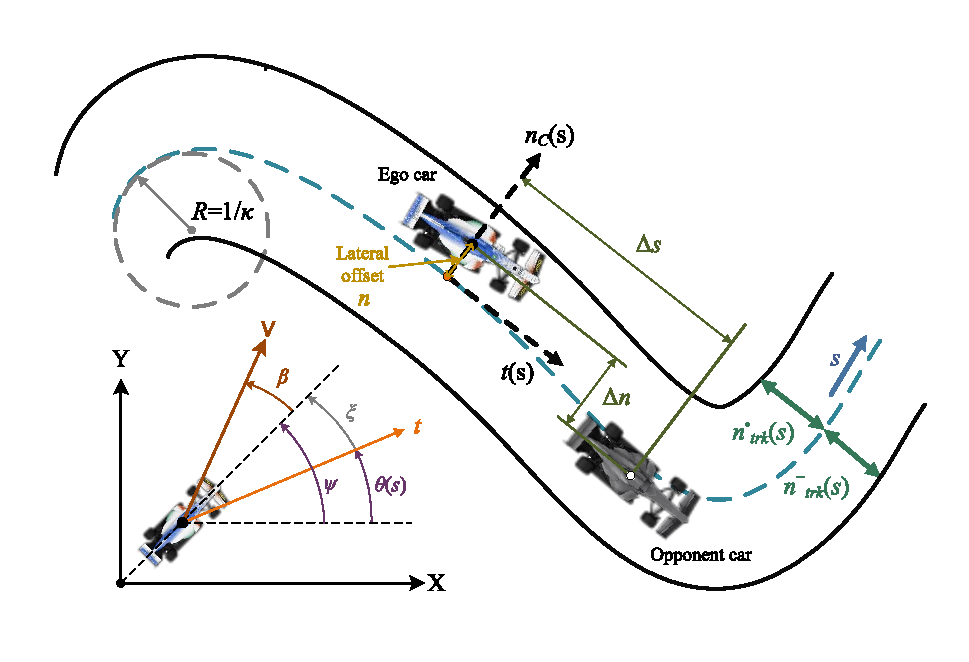
\includegraphics[width=\linewidth]{model_shuoming_corrected.pdf}
\caption{Frenet 标架下的车辆运动与相对几何关系。}
\label{fig:vehicle_track_model}
\end{figure}

将速度投影到该标架可得 $v_s=V\cos(\xi+\beta)$ 和
$v_n=V\sin(\xi+\beta)$。对式~\eqref{eq:frenet_geometry}求导得到
\begin{equation}
\begin{bmatrix}\dot s\\\dot n\\\dot\xi\end{bmatrix}
=
\begin{bmatrix}
v_s/(1-\kappa n)\\
v_n\\
r-\kappa v_s/(1-\kappa n)
\end{bmatrix}.
\label{eq:frenet_kinematics}
\end{equation}
前向正则工作域满足
$1-\kappa n\ge\varepsilon_s$，$|\xi|\le\xi_{\max}<\pi/2$，且
$v_s\ge\underline v_s>0$，数值边界见表~\ref{tab:setup_params}。对于自车--对手车对，
在起终点处展开的中心线投影定义相对状态
\begin{equation}
\begin{aligned}
g=\Delta s
&=\bigl((s_o-s_e+L_{\rm trk}/2)\bmod L_{\rm trk}\bigr)-L_{\rm trk}/2,\\
\Delta n&=n_o-n_e,\qquad
\Delta v=\dot s_e-\dot s_o,\\
\bm x_{\rm rel}&=[g,\Delta n,\Delta v]^\top,\\
\dot{\bm x}_{\rm rel}
&=
\begin{bmatrix}
-\Delta v\\
\dot n_o-\dot n_e\\
\ddot s_e-\ddot s_o
\end{bmatrix}.
\end{aligned}
\label{eq:rel}
\end{equation}
其中，$g>0$ 表示对手位于前方，$\Delta v>0$ 表示自车正在接近；这些量构成战术策略使用的
相对状态。

在空间路径生成中，规划器以 $s$ 为自变量，以 $\bm z(s)=[n(s),\xi(s)]^\top$ 为几何状态。
对于路径曲率 $\omega(s)$，精确空间模型为
\begin{equation}
\bm z'(s)=\bm f_s(\bm z,\omega;s)=
\begin{bmatrix}
(1-\kappa n)\tan\xi\\[2pt]
(1-\kappa n)\omega/\cos\xi-\kappa
\end{bmatrix}.
\label{eq:spatial_model}
\end{equation}
在每个规划站点，围绕上一迭代点的一阶近似写为
$\bm f_s\simeq\bm A_k\bm z_k+\bm B_k\omega_k+\bm b_k$，并用于
第~\ref{sec:planner}节的序列 SOCP。

% Condensed Sections 3--4: the tactical contribution is kept explicit, while
% standard execution details are summarized to preserve experimental space.

% =====================================================================
\section{博弈引导战术走廊策略}\label{sec:tactical}
% =====================================================================
所提出的策略将战术决策表示为持续可行集。响应集教师评估离线交互，TQC 蒸馏其投影动作与
价值，确定性发布器再将每个策略样本转化为供规划器使用的侧向一致走廊。

\subsection{鲁棒 Stackelberg 响应集监督}
\label{subsec:game_formulation}
在每次战术更新中，编码器将两车状态、局部赛道预瞄、当前模式、侧向锁和执行健康状态组合为
$\widetilde{\bm o}_t$。Actor 输出
\begin{equation}
\begin{aligned}
\bm a^{\rm raw}=\bigl[&L^{\rm cap},R^{\rm cap},d_{\rm safe},
V_{\rm cap}^{\rm req},g_{\rm chase},g_{\rm ot},\\
&g_{\rm abort},b_{\rm lat},w_{\rm safe},q_{\rm side}\bigr]^\top .
\end{aligned}
\label{eq:action_vec}
\end{equation}
其中，各分量依次指定可用赛道宽度、车身足迹裕量、请求速度上限、有序交互距离、防守区间和
侧向意图。欧氏投影 $\Pi_{\mathcal A}$ 强制满足表~\ref{tab:tactical_settings}中的分量边界、
门限顺序
$g_{\rm ot}+\Delta_g\le g_{\rm chase}\le g_{\rm abort}-\Delta_g$ 以及
最小走廊宽度。因此，战术动作遵循唯一映射链
\[
\bm a^{\rm raw}\xrightarrow{\Pi_{\mathcal A}}\bm a^{\rm B}
\xrightarrow{\Pi_{\rm tire}}\bm a^{\rm F},\qquad
\mathcal G_t=(m_{t+1},\sigma_{t+1}^{\rm lock},
V_{{\rm cap},t}^{\rm F},\mathcal C_t).
\]
神经策略确定战术样本；模式、侧向锁、走廊和速度上限的发布由算法~\ref{alg:tactical_corridor}
确定。

离线教师将三个侧向编码与其余动作分量上的 Sobol 设计组合，形成确定性的主车和从车候选库。
每个候选都经过与在线阶段相同的边界投影、走廊裁剪和轮胎筛选；重复或不可行候选被剔除。
令 $\mathcal A_i^G(\bm o)$ 表示角色 $i$ 的候选库。对于每个自车--对手候选对，先将角色互换的
两组预瞄插值到共同的历时域，再计算角色相对效用：
\begin{equation}
U_i(\bm o,\bm a_e^{\rm F},\bm a_o^{\rm F})=
\frac{1}{\|\bm w\|_1}\sum_{k=0}^{N_{\rm sta}-1}
\gamma_g^k\bm w^\top
\bm\phi_{i,k}(\mathcal R_e,\mathcal R_o),
\label{eq:game_utility}
\end{equation}
其中，$\bm\phi_i\in[0,1]^{10}$ 包含\ref{app:parameters}中角色互换后的奖励特征。
教师保留近最优从车响应，并以其中最不利的响应评价每个自车候选：
\begin{equation}
\begin{aligned}
U_o^{\max}(\bm o,\bm a_e^{\rm F})
&=\max_{\bm a_o^{\rm F}\in\mathcal A_o^G(\bm o)}
U_o(\bm o,\bm a_e^{\rm F},\bm a_o^{\rm F}),\\
\mathfrak R_o^\varepsilon(\bm o,\bm a_e^{\rm F})
&=\{\bm a_o^{\rm F}\in\mathcal A_o^G(\bm o):
U_o\ge U_o^{\max}-\varepsilon_{\rm BR}\},\\
\mathcal V_g(\bm o,\bm a_e^{\rm F})
&=\min_{\bm a_o^{\rm F}\in\mathfrak R_o^\varepsilon}
U_e(\bm o,\bm a_e^{\rm F},\bm a_o^{\rm F}),\\
\bm a_{\rm th}^{\star}(\bm o)
&\in\argmax_{\bm a_e^{\rm F}\in\mathcal A_e^G(\bm o)}
\mathcal V_g(\bm o,\bm a_e^{\rm F}),\\
\mathcal D_g&=\{(\widetilde{\bm o}_n,\bm a_{g,n}^{\rm F},v_{g,n}):
v_{g,n}=\mathcal V_g(\widetilde{\bm o}_n,\bm a_{g,n}^{\rm F})\}.
\end{aligned}
\label{eq:response_set_teacher}
\end{equation}
最大化结果提供响应集最优动作先验，同时每个已评估自车动作在 $\mathcal D_g$ 中保留与自身
匹配的动作条件价值标签。

参考层轮胎可接受性通过对请求速度上限进行有限搜索实现。走廊中点给出三点曲率预瞄，
第~\ref{sec:execution}节的速度扫描对有限网格
$\mathcal V_s(V_{\rm cap}^{\rm req})$ 中的每个试探值 $v$ 生成
$\widehat{\bm V}(v)$；该网格在 $V_{\min}$ 与请求上限之间均匀采样。令 $\bm a[v]$ 仅替换
候选动作中的速度上限分量。当 $\widehat a_{N,k}=\widehat\kappa_k\widehat V_k^2$ 时，投影为
\begin{equation}
\begin{aligned}
\widehat a_{T,k}(v)&=
\frac{\widehat V_{k+1}^2-\widehat V_k^2}{2\Delta\ell_k}
+a_{\rm drag}(\widehat V_k),\\
\widehat\rho(v)&=\max_k\Phi_{\rm tire}(\widehat a_{T,k}(v),
\widehat a_{N,k},\widehat V_k),\\
V_{\rm cap}^{\rm F}(\bm a)&=\max\{v\in\mathcal V_s(V_{\rm cap}^{\rm req}):
\widehat\rho(v)\le1\},\\
\Pi_{\rm tire}(\bm a;\widetilde{\bm o})
&=\bm a[V_{\rm cap}^{\rm F}(\bm a)].
\end{aligned}
\label{eq:tire_safe_action}
\end{equation}
该预瞄中的对手运动采用式~\eqref{eq:frenet_kinematics}给出的恒定 Frenet 速度。
临时走廊在搜索前构造；若搜索集合为空，发布序列首先采用当前状态的 \textsc{Hold}，必要时
进入回退。

\subsection{博弈引导的分布式策略}
\label{subsec:theory_guided_rl}
51维观测由27维双车对抗状态特征与分别以自车和对手为中心的两个12维赛道摘要拼接而成。
对抗特征包括归一化 Frenet 状态与加速度、相对进度、横向间距与接近率、碰撞时间、接近速度
编码、侧向锁以及九状态比赛模式编码。每个赛道摘要给出连续四个区间内的平均曲率、绝对曲率
峰值和最小宽度。

环境奖励为
\begin{equation}
\begin{aligned}
r_t&=\bm w^\top\bm\phi_t,\\
\bm\phi_t&=[\phi_{\rm ot},\phi_{\rm ovb},\phi_{\rm col},\phi_{\rm lat},
\phi_{\rm crush},\phi_{\rm app},\\[-1mm]
&\hspace{9mm}\phi_{\rm sm},\phi_{\rm gs},\phi_{\rm sbs},
\phi_{\rm wide}]^\top .
\end{aligned}
\label{eq:reward_sum}
\end{equation}
\ref{app:parameters}给出归一化定义与权重。角色互换后的同一组特征用于定义
式~\eqref{eq:game_utility}，从而使教师与在线奖励在超车进度、间距、平滑性和可用走廊宽度
层面保持一致。

\emph{投影动作 TQC。} 截断分位数评论家（TQC）~\cite{kuznetsov2020tqc} 在
quantile-Huber 备份前剔除最大的目标原子。环境回放池 $\mathcal D$ 存储最终战术动作
$\bm a_t^{\rm F}$。对于目标策略的原始样本，投影动作与截断目标为
\begin{equation}
\begin{aligned}
\bm a_{t+1}^{\rm F}&=\Pi_{\rm tire}\!\left(
\Pi_{\mathcal A}(\bm a_{t+1}^{\rm raw});
\widetilde{\bm o}_{t+1}\right),\\
\ell_{t+1}&=\log\pi_\theta(\bm a_{t+1}^{\rm raw}
\mid\widetilde{\bm o}_{t+1}),\\
y_{t,k}&=r_t+\gamma(1-d_t)
\left[z_{(k)}'(\widetilde{\bm o}_{t+1},\bm a_{t+1}^{\rm F})
-\alpha\ell_{t+1}\right],\\
\mathcal Y_t&=\operatorname{sg}\!\left(\{y_{t,k}\}_{k=1}^{K}\right),
\qquad K<2N_q .
\end{aligned}
\label{eq:tqc_truncated_target}
\end{equation}
因此，目标评论家与回放池具有相同的投影动作支持集，而熵仍由原始随机策略的密度计算。
Actor 与先验更新利用下式使梯度通过非光滑轮胎搜索：
\begin{equation}
\bm a^{\rm F,ST}=\bm a^{\rm B}
+\operatorname{sg}\!\left[\bm a^{\rm F}-\bm a^{\rm B}\right].
\label{eq:tire_projection_ste}
\end{equation}
该投影动作替代在前向传播中使用精确投影动作，在反向传播通过 $\Pi_{\rm tire}$ 时采用恒等映射。

两个分位数输出头共享 $\bm h_\zeta=\mathcal E_\zeta^Q(
\widetilde{\bm o},\bm a^{\rm F})$。对于匹配样本
$(\widetilde{\bm o}_g,\bm a_g^{\rm F},v_g)\sim\mathcal D_g$，令
$\bm h_{\zeta,g}=\mathcal E_\zeta^Q(
\widetilde{\bm o}_g,\bm a_g^{\rm F})$，则更新为
\begin{equation}
\begin{aligned}
\mathcal L_{\rm critic}&=J_Q+\lambda_g\,
\mathbb E_{\mathcal D_g}\!\left[
\left(g_\psi(\bm h_{\zeta,g})-\mathsf N_V(v_g)\right)^2\right],\\
\mathcal L_{\rm actor}&=J_\pi+\lambda_p\,
\mathbb E_{\widetilde{\bm o}\sim\mathcal D_g}\!\left[
\left\|\mathsf N_a(\bm\mu_\theta^{\rm F})-
\mathsf N_a(\bm a_{\rm th}^{\star})\right\|_2^2\right].
\end{aligned}
\label{eq:total_loss}
\end{equation}
其中，$J_Q$ 和 $J_\pi$ 分别为标准 TQC 评论家损失和熵正则化 Actor 损失；
$\mathsf N_a$ 与 $\mathsf N_V$ 分别对动作和教师价值进行归一化。Actor 编码器相互独立，
两个分位数头与仅训练阶段使用的鲁棒价值头共享评论家编码器。因此，$\mathcal D$ 提供
Bellman 转移，$\mathcal D_g$ 仅提供匹配的动作--价值监督。图~\ref{fig:tqc_network}概括了
训练与部署路径。

\begin{figure}[!tbp]
\centering

\includegraphics[width=\columnwidth]{tqc_network_diagram.pdf}
\caption{博弈引导 TQC 架构。青色和蓝色路径分别表示投影动作评论家与 Actor 更新，紫色路径
表示教师监督，橙色虚线箭头表示 STE 梯度路径。}
\label{fig:tqc_network}
\end{figure}

\subsection{持续意图与走廊合成}
\label{subsec:corridor_synthesis}
状态机为连续策略输出赋予时间持续性。令 $g_t$ 和 $\Delta v_t$ 为式~\eqref{eq:rel}
定义的采样相对量。当自车接近对手时锁定可行侧，并在 \textsc{Shadow} 与
\textsc{Overtake} 期间保持；仅在确认完成超车、中止或执行健康故障后释放。健康故障和中止的
优先级高于超车，完成超车的优先级高于继续超车；未锁定的自车仅在后方对手正在接近时进入
\textsc{Defend}。奖励中的超车后指示量 $P_t$ 表示连续 $N_{\rm post}$ 次更新越过超车间距阈值。

实现所选侧向的几何操作是走廊裁剪。对于
$\mathcal B_{{\rm cap},k}=[\ell_k,u_k]$，车辆足迹与单侧排除定义为
\begingroup
\setlength{\arraycolsep}{2pt}
\begin{equation}
\begin{aligned}
\rho_{{\rm exc},k}&=d_{\rm safe}+\frac12\sum_{j\in\{e,o\}}
(L_j|\sin\xi_{j,k}|+W_j|\cos\xi_{j,k}|),\\
\mathcal B_{{\rm cap},k}&=
[\max\{n_{{\rm trk},k}^{-},-R^{\rm cap}\},
\min\{n_{{\rm trk},k}^{+},L^{\rm cap}\}],\\
\mathcal C_k^{\rm side}(\sigma,\eta)&=\begin{cases}
[\ell_k+\eta[n_{o,k}+\rho_{{\rm exc},k}-\ell_k]_+,u_k],&\sigma=+1,\\
[\ell_k,u_k-\eta[u_k-n_{o,k}+\rho_{{\rm exc},k}]_+],&\sigma=-1.
\end{cases}
\end{aligned}
\label{eq:core_overtake_carver}
\end{equation}
\endgroup
其中，$\sigma=+1$ 和 $-1$ 分别选择左侧与右侧超车。\textsc{Shadow} 采用
$\eta=\operatorname{clip}((g_{\rm chase}-\widehat g_k)/
(g_{\rm chase}-g_{\rm ot}),0,1)$，\textsc{Overtake} 则在锁定侧采用完全排除
（$\eta=1$）。\textsc{Raceline} 使用受限赛道区间；\textsc{Defend} 将其与以裁剪后偏置
$n_{o,k}+b_{\rm lat}$ 为中心、宽度为 $w_{\rm safe}$ 的区间求交；\textsc{Hold} 仅保留包含
自车的连通分量。图~\ref{fig:tactical_mode_semantics}说明了这些几何含义。

\begin{figure}[!tbp]
\centering
\subfloat[\textsc{Raceline}/\textsc{Hold}.]{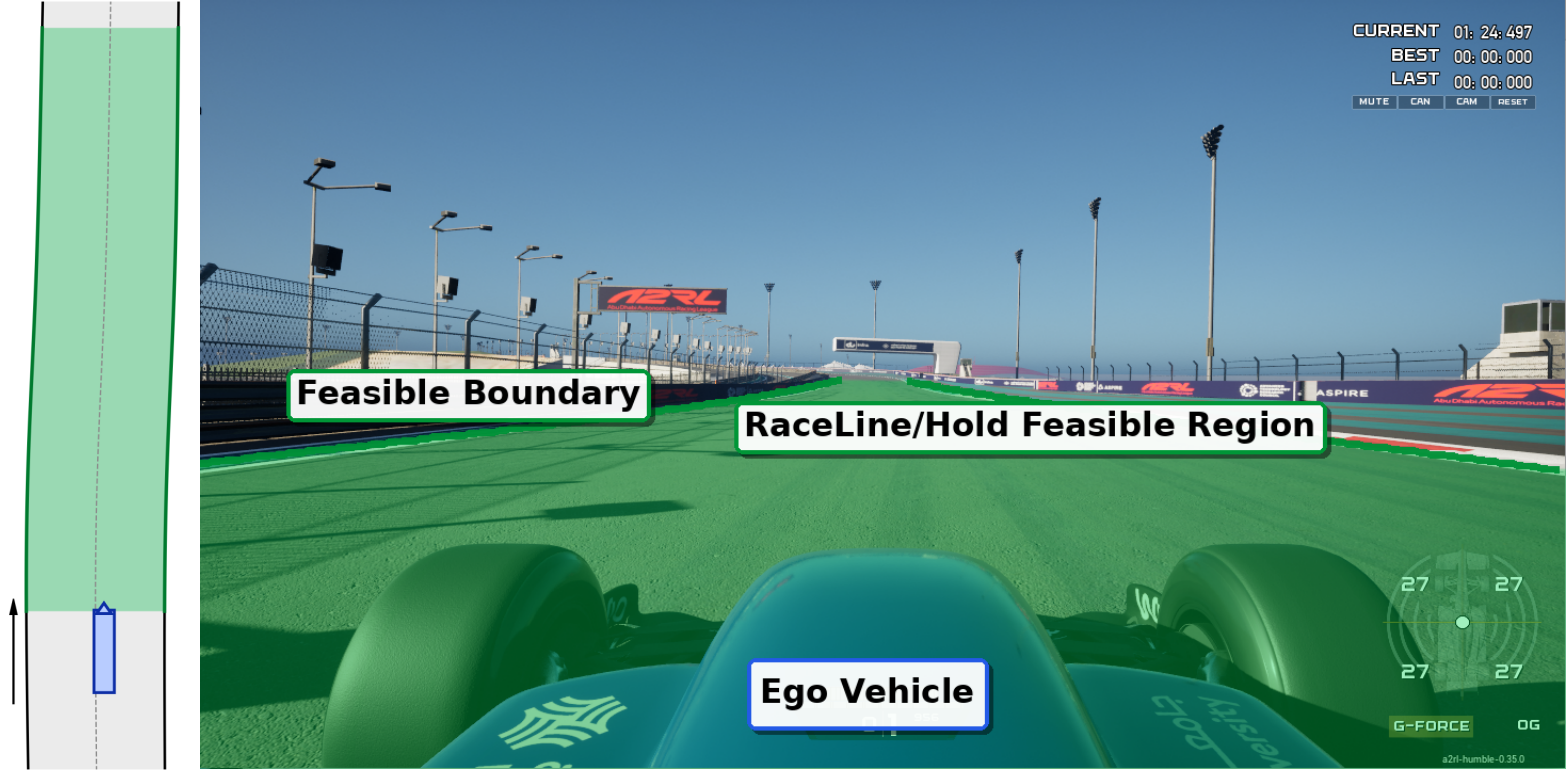
\includegraphics[width=0.48\linewidth]{race.png}}
\hfill
\subfloat[\textsc{Shadow}.]{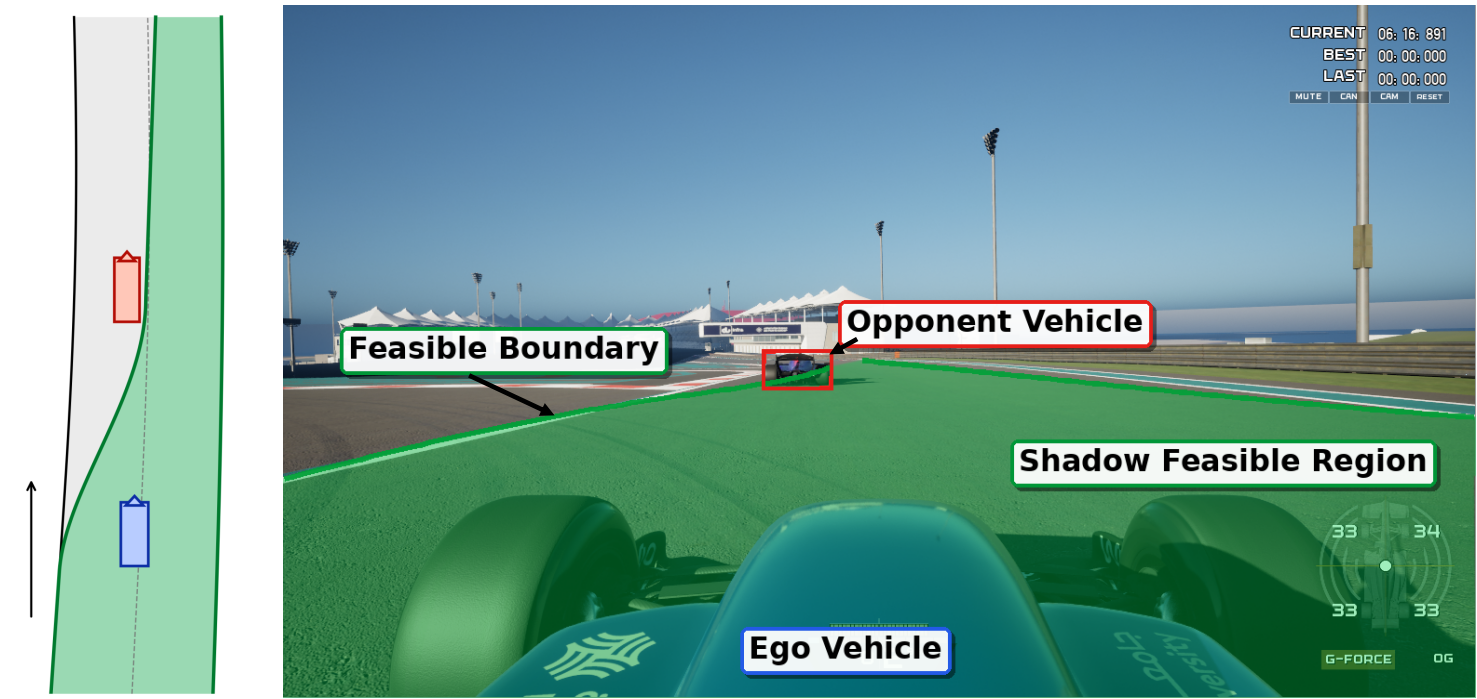
\includegraphics[width=0.48\linewidth]{shadow.png}}\\[-1mm]
\subfloat[\textsc{Overtake}.]{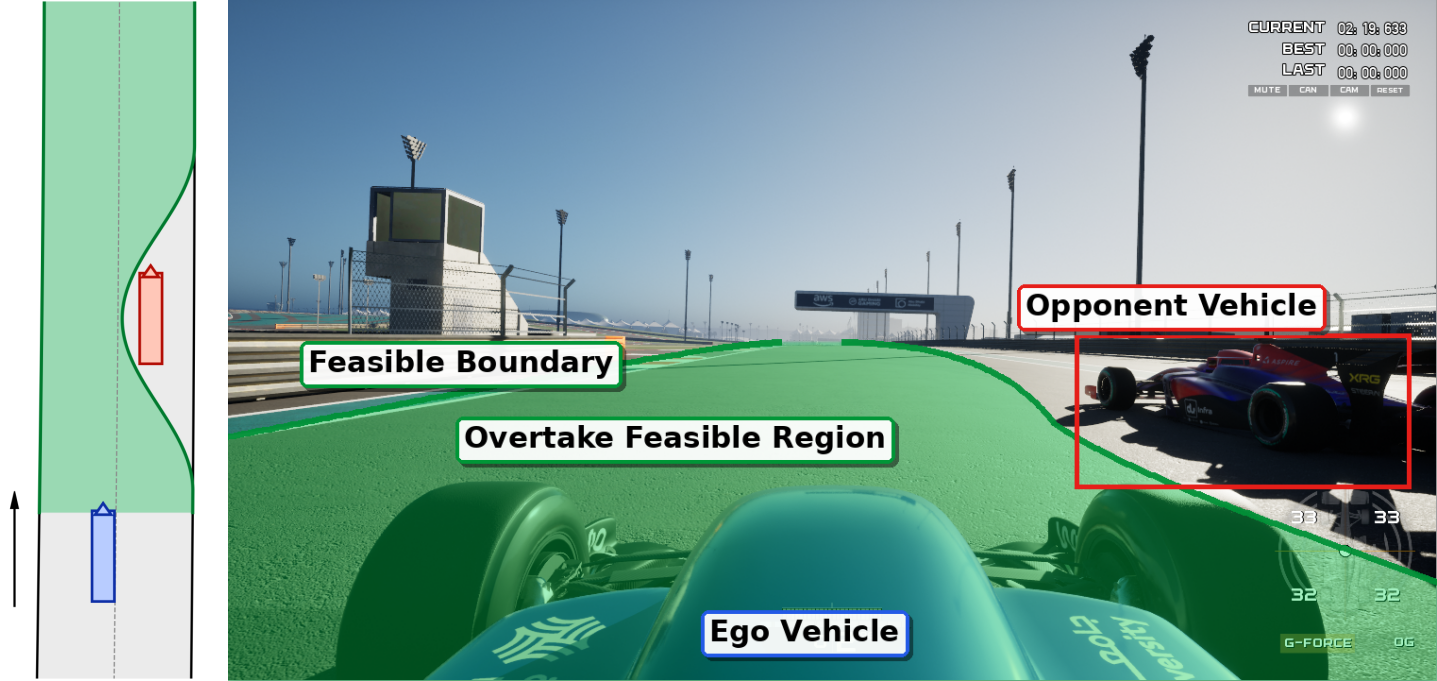
\includegraphics[width=0.48\linewidth]{overtake.png}}
\hfill
\subfloat[\textsc{Defend}.]{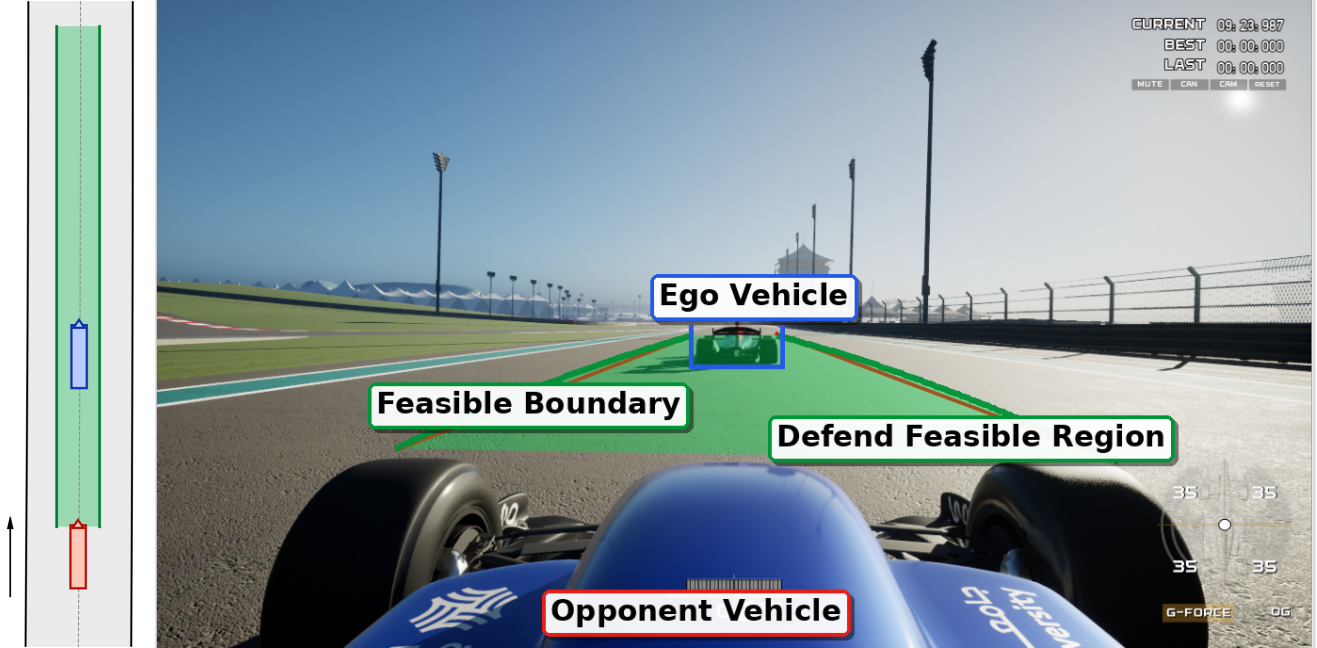
\includegraphics[width=0.48\linewidth]{defend.png}}
\caption{持续战术模式的标称几何含义。各子图将 Frenet 可行域与相应模拟器视图对应，阴影区间
为传递给规划器的区域。}
\label{fig:tactical_mode_semantics}
\end{figure}

算法~\ref{alg:tactical_corridor}汇总教师构建、学习更新和在线发布流程。在发布阶段，区间收缩
立即生效，仅对走廊放宽进行指数平滑。新建区间失效时，只有在依据当前赛道与对手重新验证后，
才允许复用上一走廊一次更新。

\begin{algorithm}[!tbp]
\caption{博弈监督的战术走廊策略}
\label{alg:tactical_corridor}
\footnotesize
\begin{algorithmic}[1]
\REQUIRE 教师状态与回放池 $\mathcal D$；在线状态、赛道预瞄、上一时刻
$(m,\sigma^{\rm lock},\mathcal C)$ 及执行健康状态
\STATE \textbf{离线教师与训练：}
\FOR{每个教师状态}
\STATE 将 Sobol 样本与左/中立/右编码组合；执行
$\bm a^{\rm raw}\!\rightarrow\!\bm a^{\rm B}\!\rightarrow\!\bm a^{\rm F}$
\STATE 剔除重复或不可行候选；在共同历时域上构造配对的角色互换预瞄
\STATE 计算式~\eqref{eq:game_utility}，保留近最优从车响应，并计算
式~\eqref{eq:response_set_teacher}
\STATE 将每个匹配的 $(\widetilde{\bm o},\bm a^{\rm F},v_g)$ 存入
$\mathcal D_g$，并保留 $\bm a_{\rm th}^{\star}$ 作为动作先验
\ENDFOR
\STATE 依据 $\mathcal D$ 更新 TQC，并依据 $\mathcal D_g$ 与式~\eqref{eq:total_loss}
更新先验/价值项
\STATE \textbf{在线战术发布：}
\STATE 采样 $\bm a^{\rm raw}$，应用 $\Pi_{\mathcal A}$，以恒定 Frenet 速度预测对手，
并评估可用侧向宽度
\IF{$h_t$ 无效，或锁定状态满足 $g_t\ge g_{\rm abort}$，或宽度小于
$L_{\min}^{\rm corr}$}
\STATE 置为 \textsc{Hold} 并释放侧向锁
\ELSIF{锁定的自车连续 $N_{\rm post}$ 次更新满足 $g_t\le-g_{\rm ot}$}
\STATE 置 $P_t=1$，返回 \textsc{Raceline} 并释放锁
\ELSIF{已存在侧向锁，或在 $0<g_t\le g_{\rm chase}$ 且 $\Delta v_t\ge0$ 时请求
非中立可行侧}
\STATE 保持/锁定该侧；当 $g_t>g_{\rm ot}$ 时选择 \textsc{Shadow}，否则选择
\textsc{Overtake}
\ELSIF{$\sigma^{\rm lock}=0$、$-g_{\rm chase}\le g_t<0$ 且 $\Delta v_t<0$}
\STATE 选择 \textsc{Defend}
\ELSE
\STATE 选择 \textsc{Raceline}
\ENDIF
\STATE 根据式~\eqref{eq:core_overtake_carver}及相应的赛车线、防守或连通保持规则构造模式区间；
\textsc{Overtake} 取 $\eta=1$，\textsc{Shadow} 采用基于间距的渐变系数
\STATE 执行有限搜索~\eqref{eq:tire_safe_action}；若为空，则重建一次当前状态
\textsc{Hold} 并重复搜索；仍为空时返回回退状态
\STATE 立即执行收缩并平滑放宽；宽度失效时最多重新验证上一走廊一次更新
\RETURN 有效时返回 $(m,\sigma^{\rm lock},V_{\rm cap}^{\rm F},\mathcal C)$；
否则返回制动回退状态
\end{algorithmic}
\end{algorithm}

% =====================================================================
\section{走廊约束规划与参考跟踪}
\label{sec:execution}\label{sec:planner}\label{sec:controller}
% =====================================================================

执行器将发布的走廊和速度上限转换为路径--速度参考及执行器指令。在站点 \(s_k\)，
\([\underline n_k,\overline n_k]\) 为按自车足迹腐蚀后的车辆中心区间。序列迭代 \(j\)
将式~\eqref{eq:spatial_model}线性化为
\(\widehat{\bm f}_{s,k}^{j}=\bm A_k^j\bm z_k+\bm B_k^j\omega_k+\bm b_k^j\)，
并求解一个走廊约束 SOCP 子问题：
\begingroup
\setlength{\arraycolsep}{2pt}
\footnotesize
\begin{equation}
\begin{aligned}
\bm y^{j+1}=\argmin_{\bm y}\;&
\sum_kw_\omega\sigma_k^\omega
+w_{n,T}\epsilon_n+w_{\xi,T}\epsilon_\xi\\
\mathrm{s.t.}\;&\bm z_0=[n_e,\xi_e]^\top,\\
&\bm z_{k+1}-\bm z_k=\frac{\Delta s_{\rm sta}}{2}
 (\widehat{\bm f}_{s,k}^{j}+\widehat{\bm f}_{s,k+1}^{j}),\\
&\underline n_k\le n_k\le\overline n_k,\quad
1-\kappa(s_k)n_k\ge\varepsilon_s,\\
&|\xi_k|\le\xi_{\max},\quad |\omega_k|\le\omega_{\max},\\
&\left\|[2\omega_k,\sigma_k^\omega-1]^\top\right\|_2
\le\sigma_k^\omega+1,\\
&|n_{N-1}-n_T|\le\epsilon_n,\quad
|\xi_{N-1}-\xi_T|\le\epsilon_\xi,\quad
\epsilon_n,\epsilon_\xi\ge0 .
\end{aligned}
\label{eq:execution_socp}
\end{equation}
\endgroup
其中，\(\bm y=\{\bm z_k,\omega_k,\sigma_k^\omega,\epsilon_n,\epsilon_\xi\}\)，
\(\bm z_k=[n_k,\xi_k]^\top\)，且
\(\omega_{\max}=\tan\delta_{\max}/(l_f+l_r)\)。在 \textsc{Raceline} 模式下，
终端目标为裁剪后的赛车线；其他模式下为走廊中点，并取 \(\xi_T=0\)。锥上图约束惩罚路径
曲率，终端松弛变量放宽向 $(n_T,0)$ 的收敛要求。每次序列更新后重新计算非线性 Frenet 模型。

对于曲率 \(\kappa_{p,k}\)，包络在 \((\kappa_{p,k}V^2,V)\) 处给出
\(a_{T,k}^{+}=[a_{T,{\rm env}}^{+}-a_{\rm drag}]_+\) 和
\(b_{T,k}^{-}=b_{T,{\rm env}}^{-}+a_{\rm drag}\)。稳态战术请求首先被转换为制动可达的
逐站上限 $V_{{\rm cap},k}^{\rm P}$。将其与包络允许的最大曲率速度求交，得到
$V_{{\rm lim},k}=\min\{\overline V_{{\rm curv},k},
V_{{\rm cap},k}^{\rm P}\}$。相应的前向--后向扫描为
\begin{equation}
\begin{aligned}
V_0^f&=V_e,\\
V_{k+1}^{f}&=\operatorname{clip}_{[V_{\min},V_{{\rm lim},k+1}]}
\sqrt{(V_k^f)^2+2\Delta\ell_k a_{T,k}^{+}(V_k^f)},\\
V_{N-1}^r&=\min\{V_{N-1}^{f},V_{{\rm lim},N-1}\},\\
V_k^r&=\min\left\{V_k^f,V_{{\rm lim},k},
\sqrt{(V_{k+1}^r)^2+
2\Delta\ell_k b_{T,k+1}^{-}(V_{k+1}^r)}\right\}.
\end{aligned}
\label{eq:execution_speed_sweep}
\end{equation}
前向扫描从实测速度开始，后向扫描保证下游制动可达性。对 $1/V_k^r$ 进行梯形积分，得到在
控制器网格上重采样路径--速度参考所需的时间戳。

RC-NMPC 在固定预测网格上跟踪重采样后的路径--速度参考。其状态与输入分别为
$\bm\chi_k=[x_k,y_k,\theta_k]^\top$ 和 $\bm\nu_k=[V_k,\delta_k]^\top$。
控制器求解
\begin{equation}
\begin{aligned}
\min_{\{\bm\nu_k\}}\;&q_{\Delta\delta}(\delta_0-\delta_{-1})^2+
\sum_{k=0}^{N_c-1}\!\left(q_ce_{c,k+1}^2+q_\psi e_{\psi,k+1}^2\right.\\[-1mm]
&\left.\hspace{30mm}+\bm e_{\nu,k}^\top\bm R_\nu\bm e_{\nu,k}\right)\\
\mathrm{s.t.}\;&\bm\chi_0=\bm0,\quad
\bm\chi_{k+1}=\bm\chi_k+T_c
\begin{bmatrix}
V_k\cos\theta_k\\ V_k\sin\theta_k\\
V_k\tan\delta_k/(l_f+l_r)
\end{bmatrix},\\
&V_{\min}\le V_k\le
\min\{v_{x,\max},V_{{\rm cap},t,k}^{\rm C}\},\quad
|\delta_k|\le\delta_{\max},\\
&|V_k-V_{k-1}|\le\Delta V_{\max},\quad
|\delta_k-\delta_{k-1}|\le\dot\delta_{\max}T_c .
\end{aligned}
\label{eq:execution_mpcc}
\end{equation}
其中，$\bm\nu_k^r=[V_k^r,\delta_k^r]^\top$，且
$\delta_k^r=\arctan((l_f+l_r)\kappa_{p,k}^r)$。变量
$e_{c,k}=(\bm n_k^r)^\top(\bm p_k-\bm p_k^r)$,
$e_{\psi,k}=\operatorname{wrap}(\theta_k-\theta_k^r)$ 和
$\bm e_{\nu,k}=\bm\nu_k-\bm\nu_k^r$ 分别为轮廓、航向与输入跟踪误差。逐阶段上限
$V_{{\rm cap},t,k}^{\rm C}$ 由上一速度指令对稳态战术请求进行速率限制得到。实际轮胎需求见
第~\ref{sec:experiments}节。

\begin{algorithm}[!tbp]
\caption{通用参考生成器与执行器}
\label{alg:executor}
\footnotesize
\begin{algorithmic}[1]
\REQUIRE 引导量 \(\mathcal G_t\)、当前状态、上一有效参考
\STATE 按自车足迹腐蚀赛道，与 $\mathcal C_t$ 求交，并选择模式相关的终端目标
\STATE 由上一有效解或走廊中点初始化空间路径
\FOR{每次设定的序列凸化迭代}
\STATE 求解 SOCP~\eqref{eq:execution_socp}，更新线性化点，并计算非线性 Frenet 与走廊残差
\STATE 当求解器状态及\ref{app:parameters}中的残差容差满足要求时停止
\ENDFOR
\STATE 若路径通过求解器、工作域和残差检查，则置为有效
\IF{有效}
\STATE 查询 $\mathcal A_{\rm tire}(V)$，根据 $V_{\rm cap}^{\rm F}$、实测速度和可用制动能力
构造 $V_{{\rm cap},k}^{\rm P}$
\STATE 将 $V_{{\rm cap},k}^{\rm P}$ 与曲率--速度包络求交，执行
式~\eqref{eq:execution_speed_sweep}，并依据轮胎检查更新有效状态
\ENDIF
\IF{有效}
\STATE 对路径--速度参考进行时间重采样，并对 $V_{{\rm cap},t}^{\rm F}$ 限速率以得到
$V_{{\rm cap},t,k}^{\rm C}$
\STATE 求解 RC-NMPC~\eqref{eq:execution_mpcc}，并根据其状态更新有效性
\ENDIF
\IF{有效}
\STATE 将 $(V_{0|t}^{c\star},\delta_{0|t}^{c\star})$ 映射为油门、制动、转向和挡位
\ELSE
\STATE 对上一参考重新验证一个周期；否则请求当前状态 \textsc{Hold}，并使用上一转向角输出
限速率制动
\ENDIF
\RETURN 四通道指令与健康状态
\end{algorithmic}
\end{algorithm}
\FloatBarrier
\endgroup
\section{实验结果与分析}\label{sec:experiments}
% =====================================================================

\subsection{实验平台与配置}
\label{subsec:hil_env}\label{subsec:param_setup}

完整的战术、规划、控制与执行器分配算法栈运行于 A2RL EAV24 平台安装的 Neousys
RGS-8805GC 工业计算机~\cite{a2rl2024,hoffmann2026a2rl,neousysrgs}。EAV24 被控对象与
Yas Marina 环境运行在独立服务器上（图~\ref{fig:a2rl_sim}）。自车、对手和赛事控制状态
通过两路虚拟 CAN 通道进入目标计算机；油门百分比、制动压力、转向执行器位置和请求挡位
通过同一车辆接口返回，ROS~2 数据流同步记录车辆与算法状态。

\begin{figure}[!tbp]
\centering

\includegraphics[width=\linewidth]{sim_shuoming.pdf}
\caption{目标硬件在环拓扑。RGS-8805GC 执行完整算法，并通过双 CAN 通道与 EAV24 被控对象
交换车辆状态和四通道执行器指令。}
\label{fig:a2rl_sim}
\end{figure}

所配置的被控对象包含六挡映射动力总成以及受速率限制的油门、制动和转向执行器，同时建模
悬架、防侧倾、空气动力、轮胎松弛、滚动阻力、车轮惯量、热效应和碰撞效应。自车与对手状态
以100~Hz生成，GNSS/姿态以100~Hz生成，IMU数据以250~Hz生成，控制器以20~Hz运行。
模拟器提供的车辆状态输入战术算法栈，使硬件在环评估聚焦于交互决策、优化、目标硬件时序、
CAN传输和执行器实现。所有方法均在相同被控对象、赛道、规划器、RC-NMPC和执行器配置下
评估1000圈闭环运行。

以一圈闭环运行作为汇总分析单元。超车成功率（OSR）定义为：在评估时域内，自车在保持横向
间距的同时改变纵向次序的圈数占比。超车时间（TTO）、最小车间距、碰撞次数、平均碰撞时间
（TTC）、赛道边界违规率和路径可行率（PFR）用于衡量战术有效性与闭环执行效果。OSR报告
双侧95\%精确二项置信区间；配对成功次数采用带Holm校正的双侧两比例$z$检验比较；五个独立
训练策略用于给出种子层面的OSR均值和标准差。

\subsection{典型赛道工况下的超车性能}
\label{subsec:representative_cases}

图~\ref{fig:four_case_track_overview}展示了 Yas Marina 赛道不同位置的四种超车情形。
空间视图将已发布走廊与规划路径同同步的 \textsc{Shadow} 和 \textsc{Overtake} 模拟器画面
对应，表明同一战术接口能够适用于不同局部几何与交互构型。工况I和II分别代表短窗口高速接近
与持续急弯交互，因此对其进行详细分析。

\begin{figure*}[!t]
\centering
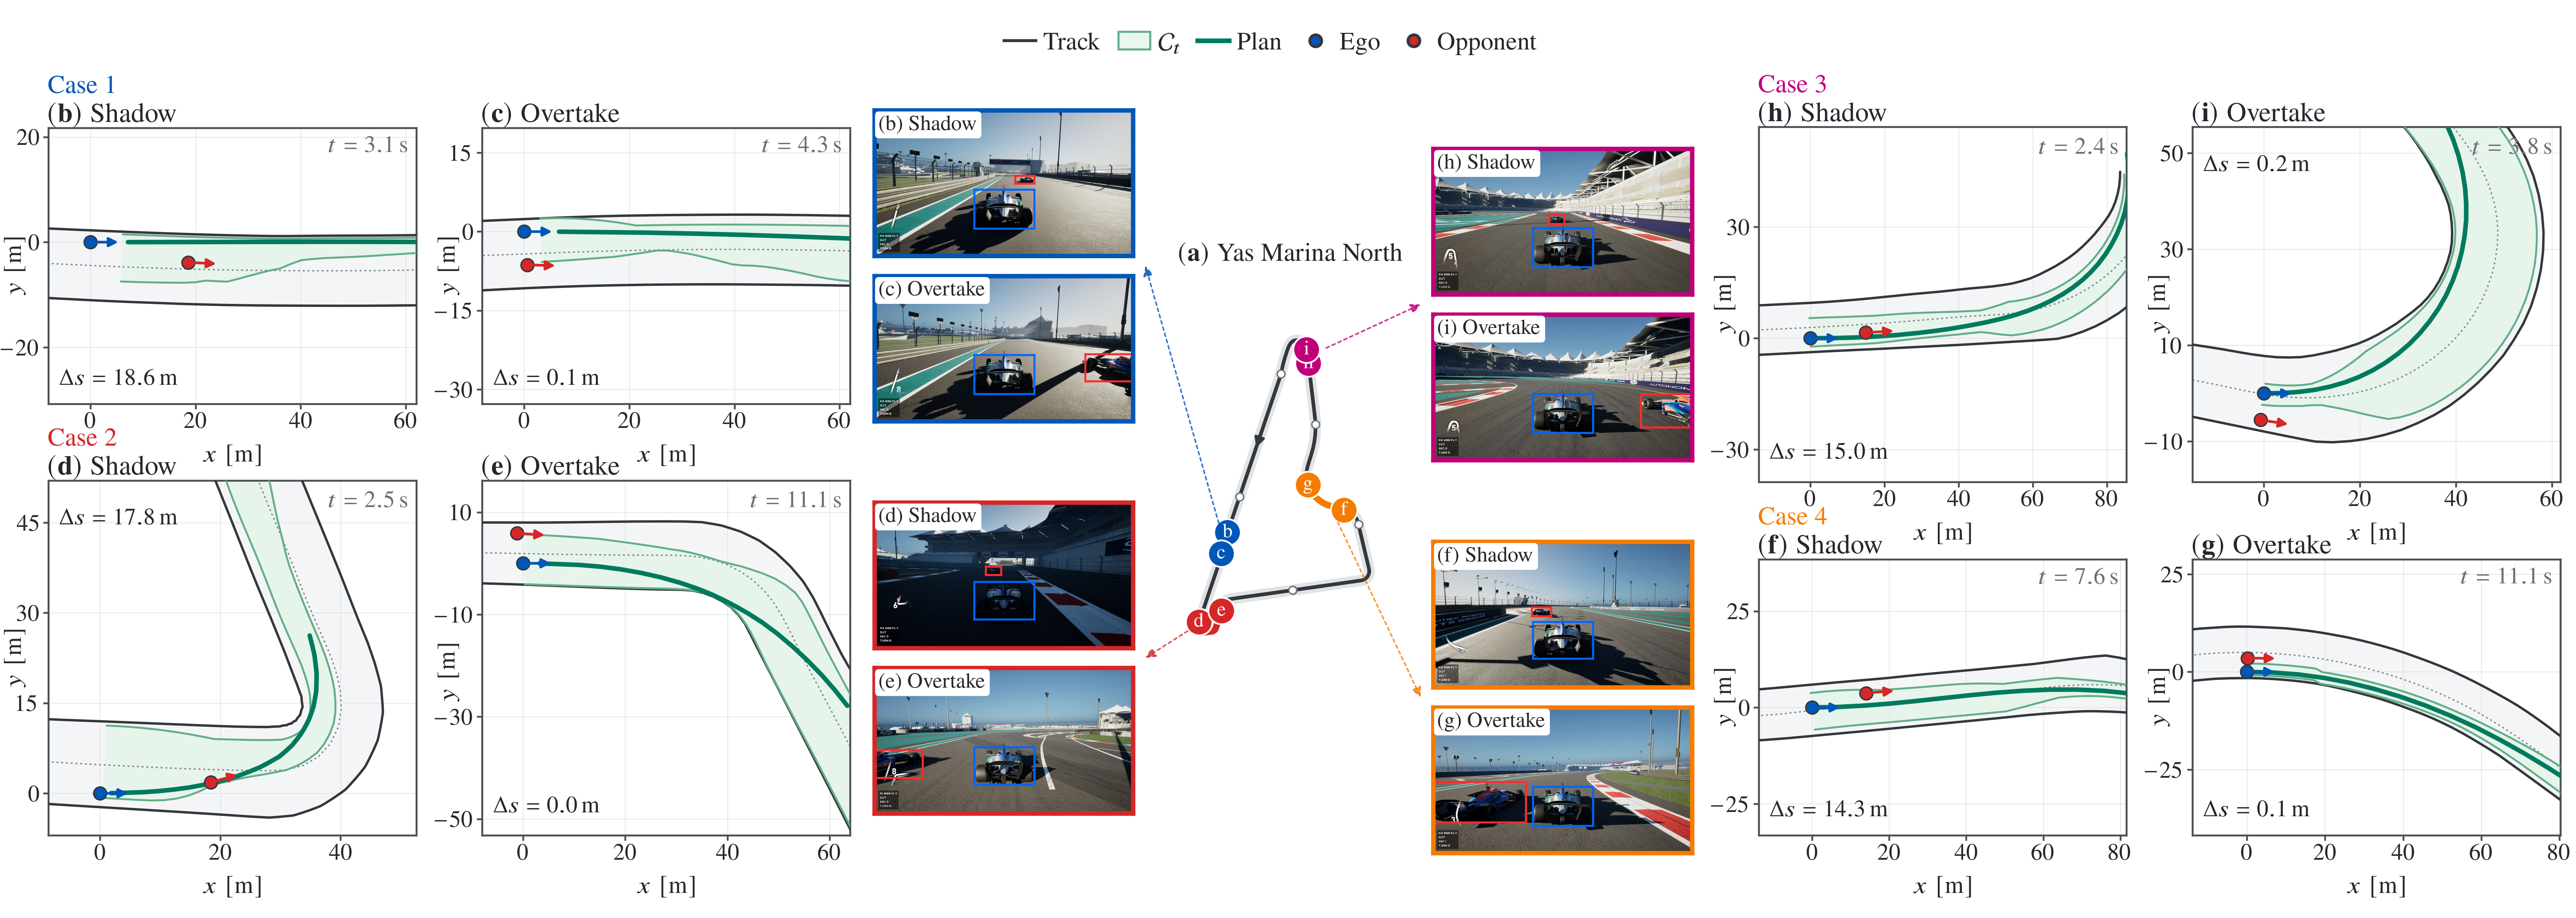
\includegraphics[width=\textwidth]{track_overview_case0205_v018.png}
\caption{Yas Marina 赛道上的典型超车情形。各彩色位置将空间走廊和规划路径与同步的
\textsc{Shadow}、\textsc{Overtake} 模拟器视图对应。}
\label{fig:four_case_track_overview}
\end{figure*}

\subsubsection*{工况I：短决策窗口下的高速超车}

工况I以约69~m~s$^{-1}$开始，对手速度明显较低，可用于锁定机动的窗口较短。
图~\ref{fig:case02_tactical_new}给出了从 \textsc{Raceline} 经 \textsc{Shadow} 到
\textsc{Overtake} 的有序转换。发布走廊始终位于物理赛道边界内，并从接近至完成超车提供连续
横向通道；自车优化路径利用该通道建立并保持与对手的间隔。同时，实际速度跟踪期望剖面，
并在超车过程中超过70~m~s$^{-1}$，验证了本文最高速代表工况下的战术执行能力。

\begin{figure}[!tbp]
\centering
\subfloat[FSM模式序列。]{
\includegraphics[width=\linewidth]{other_pic_V18/single_panels/case_02_fsm_mode.png}}\\[-0.5mm]
\subfloat[路径、走廊与赛道边界。]{
\includegraphics[width=\linewidth]{other_pic_V18/single_panels/case_02_path_corridor.png}}\\[-0.5mm]
\subfloat[车速响应。]{
\includegraphics[width=\linewidth]{other_pic_V18/single_panels/case_02_dynamics_speed.png}}
\caption{工况I的战术与速度演化。(a) FSM建立持续超车阶段；(b)规划路径保持在发布走廊和物理
赛道边界内；(c)接近对手时，实际速度在70~m~s$^{-1}$以上跟踪期望剖面。}
\label{fig:case02_tactical_new}
\end{figure}

图~\ref{fig:case02_tracking_new}中的闭环响应表明，高速走廊在整个超车过程中均可跟踪。
横向、速度和航向误差集中于零附近，仅在交互事件处出现短暂瞬态；完整加速度序列也始终位于
随速度变化的轮胎需求包络内。结合速度响应可以看出，侧向锁定走廊在高速超车中保持了跟踪
精度和参考层轮胎可接受性。

\begin{figure}[!tbp]
\centering
\subfloat[横向轮廓误差。]{
\includegraphics[width=\linewidth]{other_pic_V18/single_panels/case_02_tracking_lateral.png}}\\[-0.5mm]
\subfloat[速度跟踪误差。]{
\includegraphics[width=\linewidth]{other_pic_V18/single_panels/case_02_tracking_speed.png}}\\[-0.5mm]
\subfloat[航向跟踪误差。]{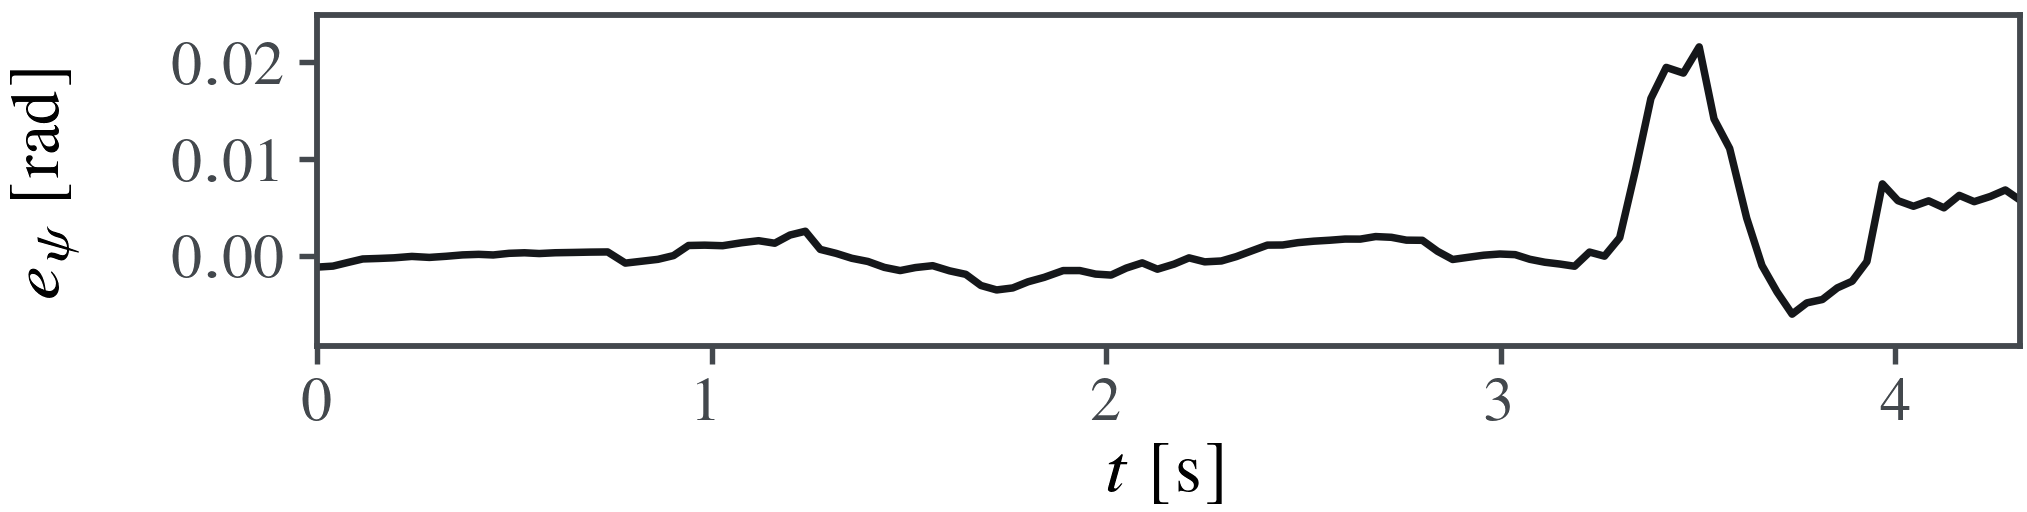
\includegraphics[width=\linewidth]{other_pic_V18/single_panels/case_02_tracking_heading.png}}\\[-0.5mm]
\subfloat[实际加速度需求。]{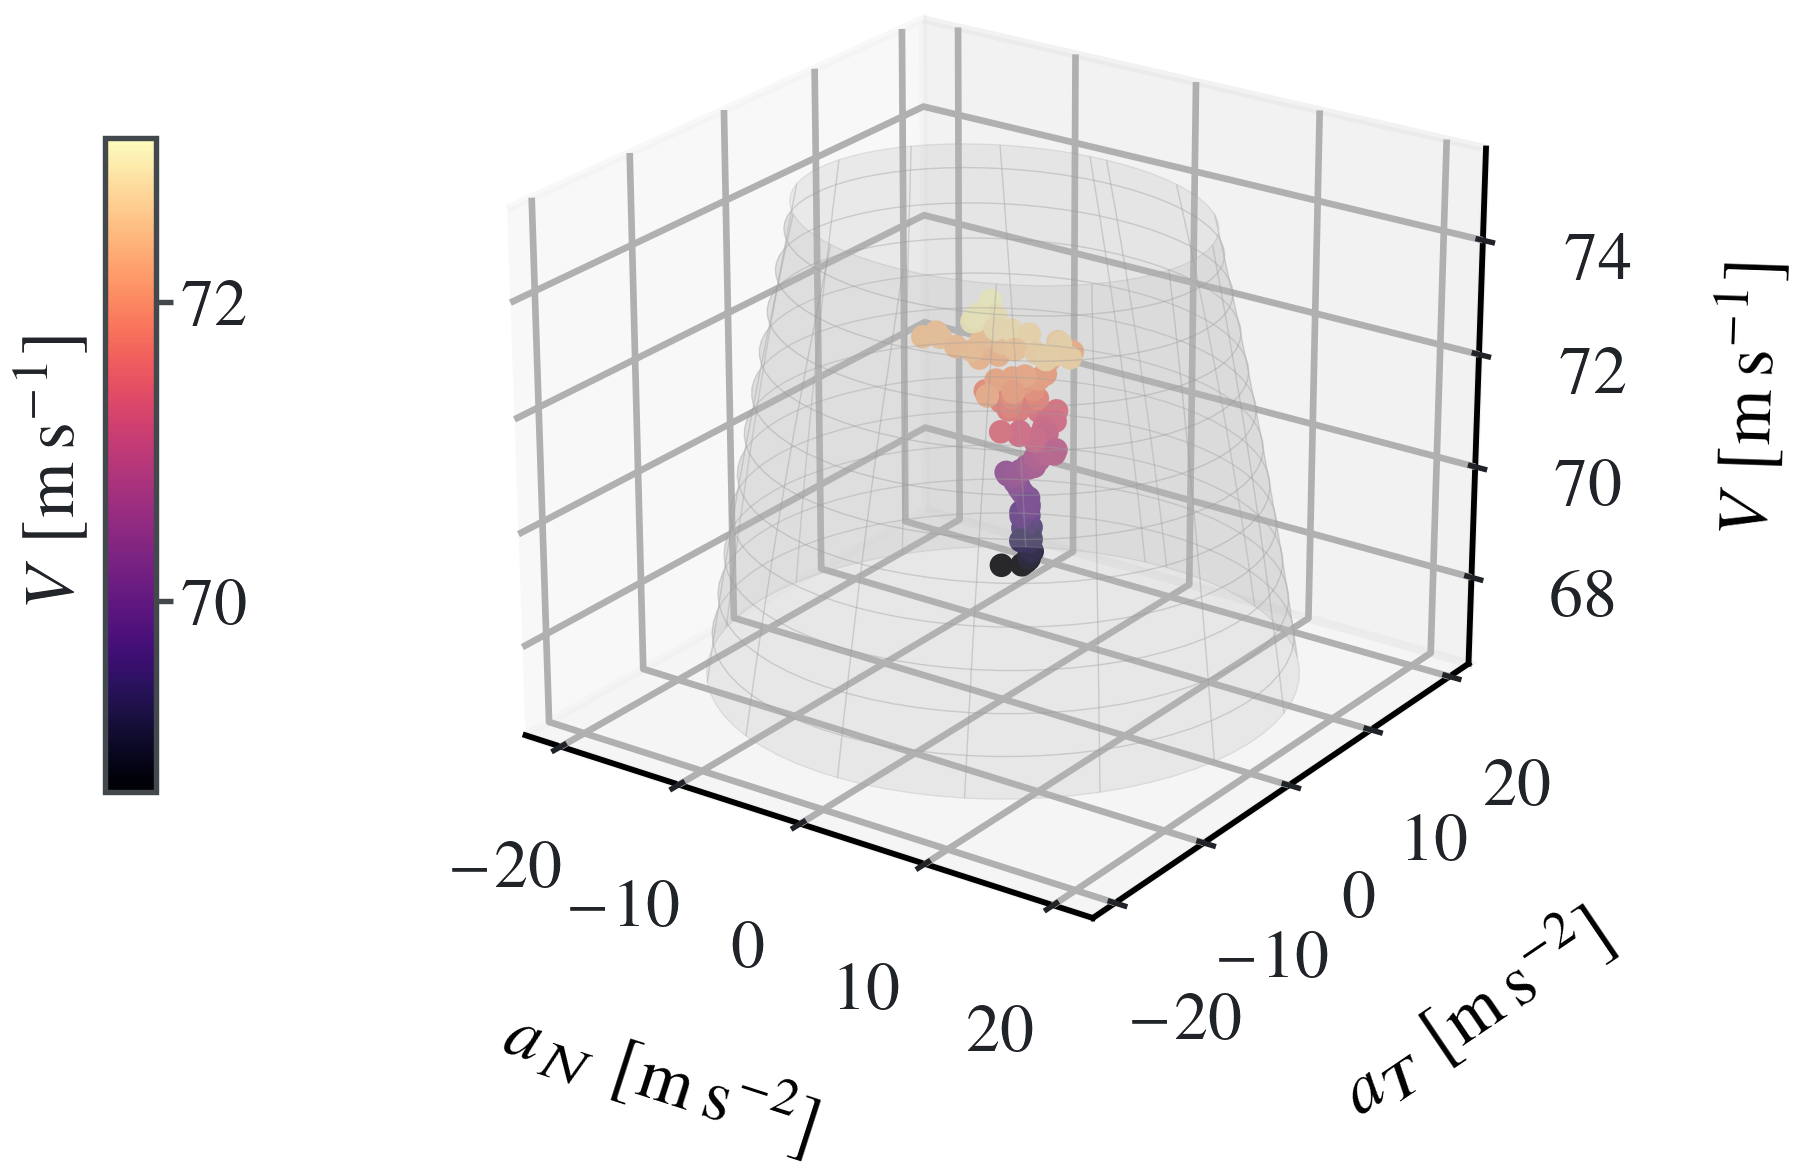
\includegraphics[width=\linewidth]{other_pic_V18/single_panels/case_02_gg_diagram.png}}
\caption{工况I的闭环跟踪与轮胎需求响应。(a--c)横向、速度和航向误差在战术切换及超车过程中
保持有界；(d)所有记录的切向--法向加速度样本均位于给定的随速度变化轮胎需求包络内。}
\label{fig:case02_tracking_new}
\end{figure}

\subsubsection*{工况II：连续急弯中的持续超车}

工况II的入弯速度超过60~m~s$^{-1}$，并在连续曲率变化中形成更长时间的交互。
图~\ref{fig:case05_tactical_new}表明，FSM首先建立 \textsc{Shadow}，随后锁定
\textsc{Overtake} 直至机动结束。所示站点处的物理边界变化明显，但裁剪器在可用赛道宽度内
保持连通走廊，规划路径在交互与超车标记之间始终位于走廊内。速度响应跟踪入弯制动剖面，
随后重新加速至35~m~s$^{-1}$以上，从而在高曲率序列中持续保持超车机会。

\begin{figure}[!tbp]
\centering
\subfloat[FSM模式序列。]{
\includegraphics[width=\linewidth]{other_pic_V18/single_panels/case_05_fsm_mode.png}}\\[-0.5mm]
\subfloat[路径、走廊与赛道边界。]{
\includegraphics[width=\linewidth]{other_pic_V18/single_panels/case_05_path_corridor.png}}\\[-0.5mm]
\subfloat[车速响应。]{
\includegraphics[width=\linewidth]{other_pic_V18/single_panels/case_05_dynamics_speed.png}}
\caption{工况II的战术与速度演化。(a) FSM在弯道交互中保持所选超车侧；(b)规划路径与发布
走廊始终位于变化的物理赛道边界内；(c)实际速度跟踪期望制动与再加速剖面。}
\label{fig:case05_tactical_new}
\end{figure}

由于制动、转弯和相对位置变化同时发生，更急的几何条件产生了比工况I更大的瞬态误差
（图~\ref{fig:case05_tracking_new}）。每次曲率切换后，横向和航向误差均回归零附近，
速度跟踪在制动与再加速过程中保持有界；在全部记录速度范围内，加速度样本均位于轮胎包络内。
因此，两种工况形成互补证据：学习走廊既支持70~m~s$^{-1}$以上的超车，也支持受限弯道序列
中的持续超车。

\begin{figure}[!tbp]
\centering
\subfloat[横向轮廓误差。]{
\includegraphics[width=\linewidth]{other_pic_V18/single_panels/case_05_tracking_lateral.png}}\\[-0.5mm]
\subfloat[速度跟踪误差。]{
\includegraphics[width=\linewidth]{other_pic_V18/single_panels/case_05_tracking_speed.png}}\\[-0.5mm]
\subfloat[航向跟踪误差。]{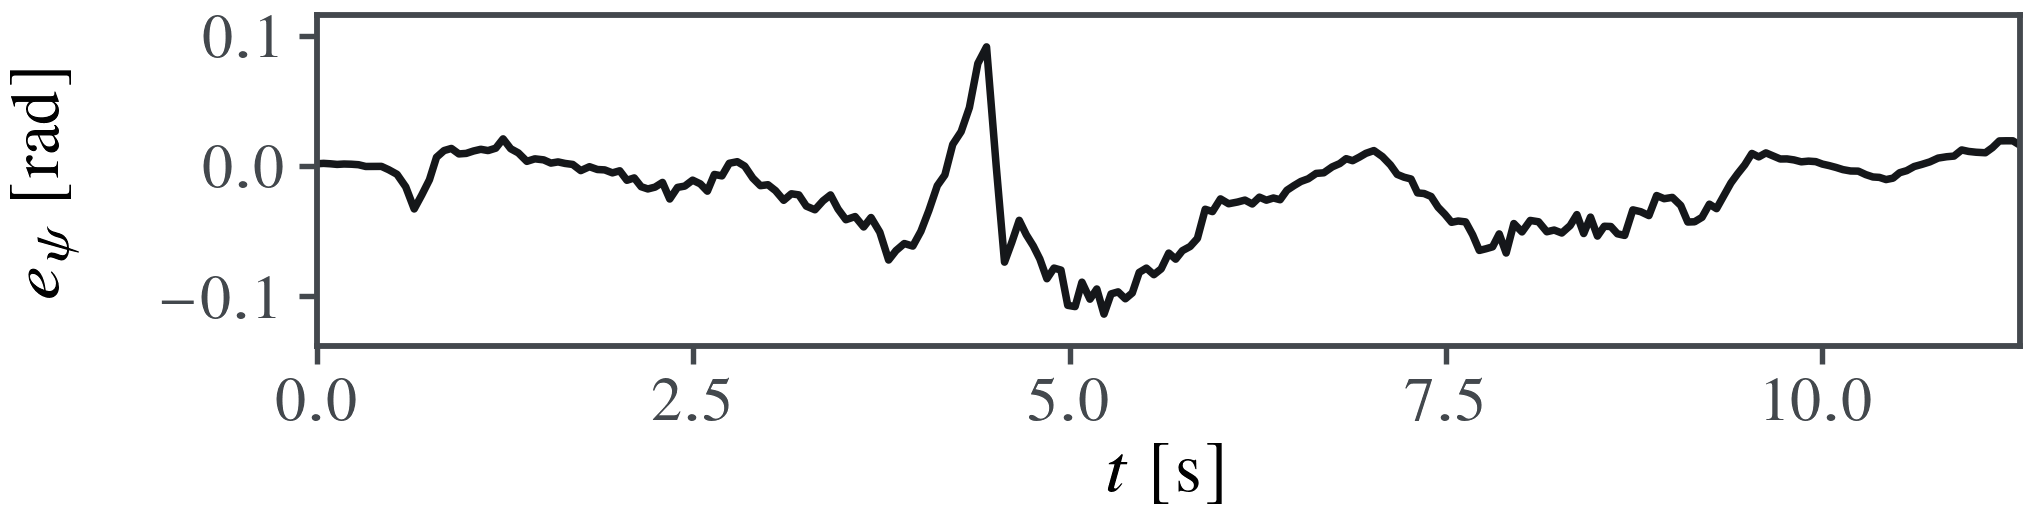
\includegraphics[width=\linewidth]{other_pic_V18/single_panels/case_05_tracking_heading.png}}\\[-0.5mm]
\subfloat[实际加速度需求。]{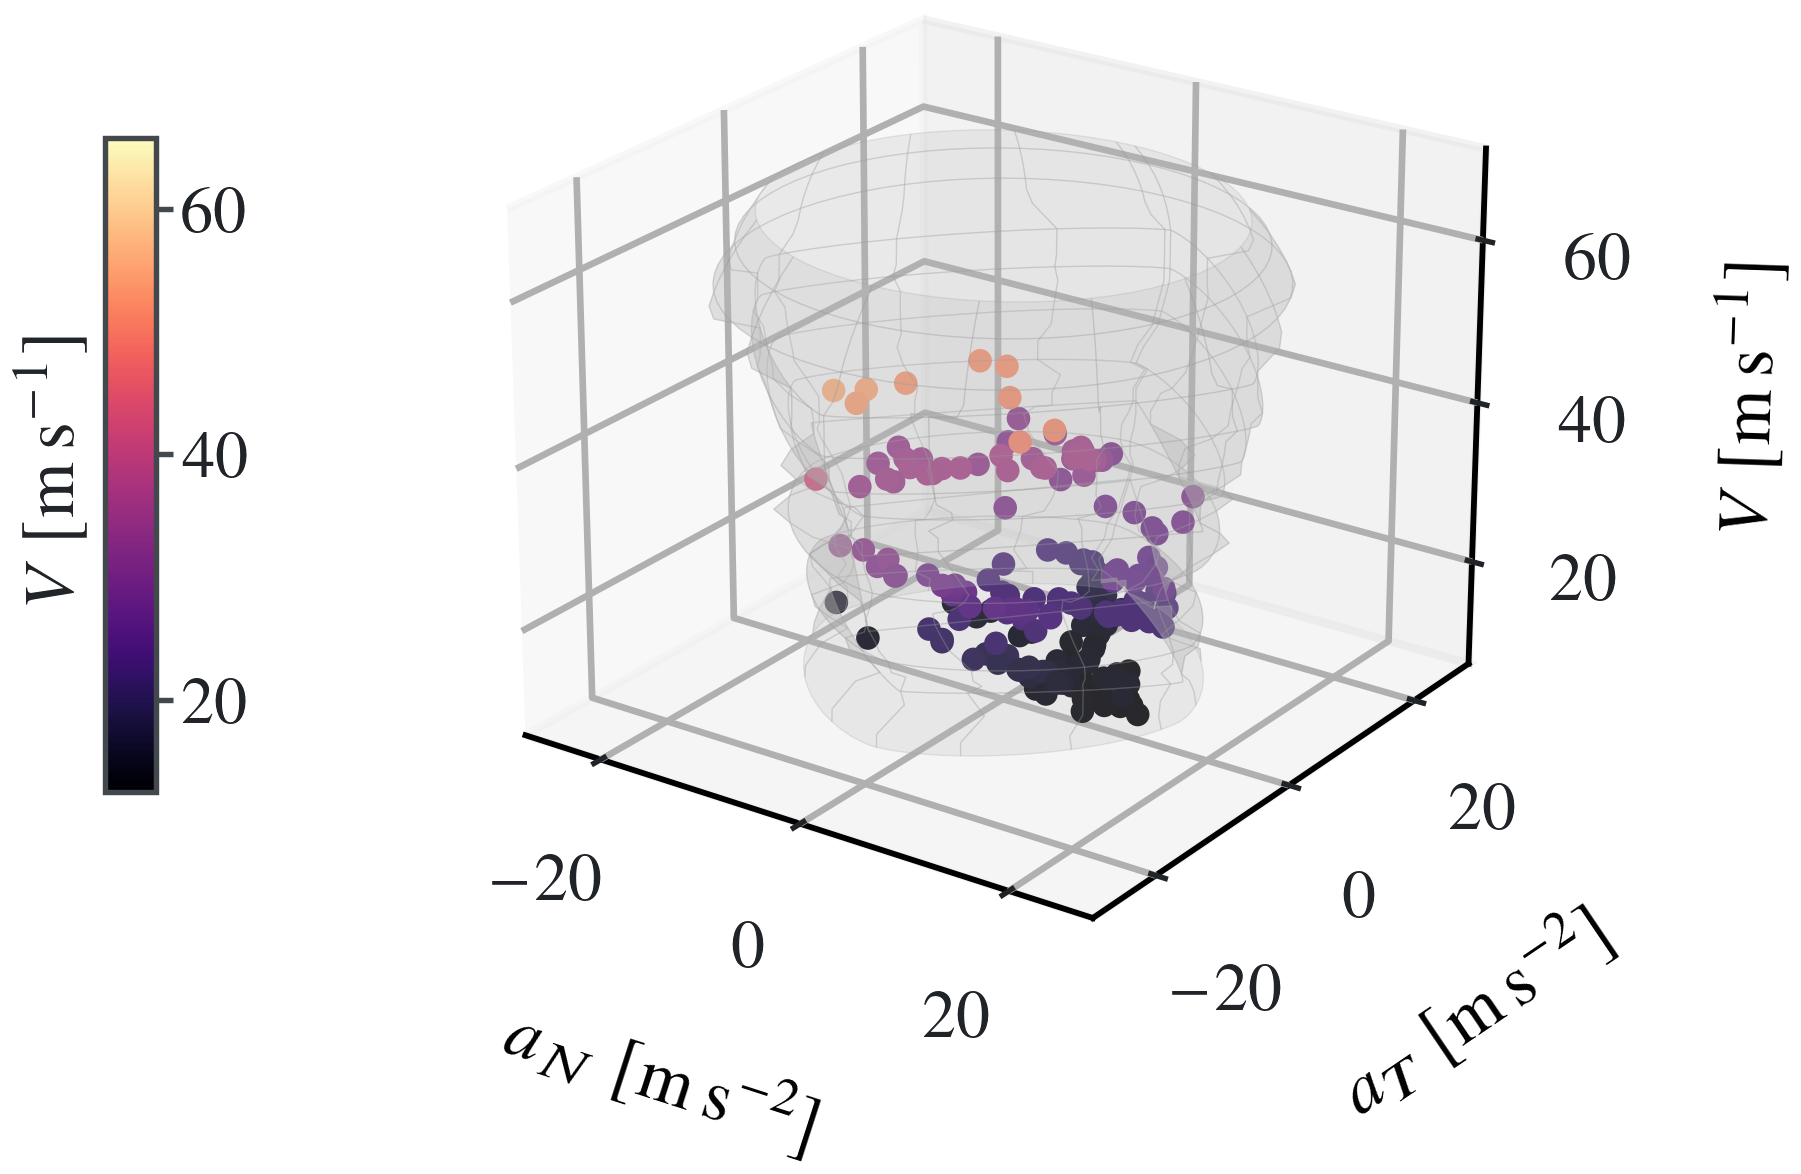
\includegraphics[width=\linewidth]{other_pic_V18/single_panels/case_05_gg_diagram.png}}
\caption{工况II的闭环跟踪与轮胎需求响应。(a--c)跟踪误差在持续弯道交互的制动、转向与出弯
阶段保持有界；(d)所有记录的加速度样本均位于给定的随速度变化轮胎需求包络内。}
\label{fig:case05_tracking_new}
\end{figure}

在重复评估中，完整方法在1000圈中成功完成947圈（OSR为94.7\%，95\%精确二项置信区间为
93.1--96.0\%），且未观察到碰撞或赛道边界违规。五个独立训练策略的种子层面OSR为
$94.3\%\pm0.7\%$（均值$\pm$标准差）。下文的配对比较用于量化交互战术表示及其组成模块
的贡献。

% =====================================================================
% Matched comparison and ablation results
% =====================================================================

\subsection{与战术基线的比较}
\label{subsec:comparison}

所有方法采用相同的被控对象、赛事控制接口、走廊投影、路径与速度规划器、RC-NMPC 和执行器
分配器，仅战术引导模块不同。\emph{Pure Raceline} 跟踪标称赛车线；
\emph{Non-Interactive MPC} 独立于自车规划预测对手，并在结果上施加障碍物约束
~\cite{kabzan2020amzracing,betz2023autonomous}；\emph{Rule-based GT} 使用固定阈值状态机
（$g_{\rm chase}=20$ m，$g_{\rm ot}=8$ m，$g_{\rm abort}=35$ m）；\emph{iLQGames}
通过迭代线性二次博弈近似计算耦合局部响应~\cite{fridovich2020ilqgames}。所有基线输出均
投影到相同的侧向、速度上限和走廊接口，从而形成战术推理的配对比较。

\begin{table}[!tbp]
\centering
\footnotesize
\setlength{\tabcolsep}{2.3pt}
\renewcommand{\arraystretch}{1.08}
\caption{各方法1000圈闭环硬件在环实验的配对比较。箭头表示指标的优选方向。}
\label{tab:comparison}
\begin{tabular}{@{}lccccc@{}}
\toprule
指标 & 本文 & PR & NI-MPC & RB-GT & iLQG \\
\midrule
OSR [\%] $\uparrow$             & \textbf{94.7} & 38.2 & 28.5 & 51.6 & 63.5 \\
OSR差值 [pp] $\downarrow$      & \textbf{0.0} & 56.5 & 66.2 & 43.1 & 31.2 \\
TTO [s] $\downarrow$            & \textbf{4.82} & 7.25 & 11.23 & 9.37 & 7.83 \\
最小间距 [m] $\uparrow$         & \textbf{5.83} & 1.42 & 3.85 & 2.14 & 2.31 \\
碰撞 [次] $\downarrow$      & \textbf{0} & 21 & 7 & 48 & 14 \\
平均TTC [s] $\uparrow$         & \textbf{8.52} & 3.21 & 6.92 & 5.64 & 5.73 \\
越界率 [\%] $\downarrow$  & \textbf{0.0} & \textbf{0.0} & \textbf{0.0} & \textbf{0.0} & \textbf{0.0} \\
PFR $\uparrow$                  & \textbf{1.000} & 0.988 & 0.998 & 0.987 & 0.995 \\
\bottomrule
\end{tabular}
\vspace{1mm}

\begin{minipage}{\columnwidth}
\scriptsize
\emph{注：}PR表示纯赛车线，NI-MPC表示非交互式MPC，RB-GT表示基于规则的博弈策略，
iLQG表示iLQGames。OSR差值为相对于本文方法的百分点差；最小间距为逐圈最小车间距的均值；
PFR为获得可行SOCP解的规划周期占比。粗体表示观测到的最优值；相同的越界率均加粗。
\end{minipage}
\end{table}

表~\ref{tab:comparison}通过OSR及其差值直接体现主要效果。所提出的战术走廊策略完成94.7\%
的测试圈，比最强基线iLQGames高31.2个百分点，同时未发生碰撞，并在每个规划周期保持路径
可行。iLQGames在基线中表现最佳，验证了耦合交互推理的作用；在此基础上，本文持续走廊将
OSR由63.5\%提高至94.7\%，并将碰撞由14次降至0次。非交互式MPC保持了相对较大的最小间距，
但仅完成28.5\%的超车；本文策略同时将最小间距提高至5.83~m，并取得94.7\%的OSR。基于规则
的方法在不同曲率和相对速度条件下发生48次碰撞。总体而言，响应集教师与持续可行域接口兼顾
面向对手的机会选择、间距保持和可靠闭环执行。

对四组OSR比较采用带Holm校正的双侧两比例$z$检验，校正后均有$p<10^{-6}$，与
表~\ref{tab:comparison}中的效应量和事件次数所反映的差异一致。

\subsection{消融实验}
\label{subsec:ablation}

在保持执行层相同的条件下，四组消融分别隔离所提出的战术组件。\emph{无博弈引导（No-GG）}
同时移除Stackelberg响应集动作先验和动作条件鲁棒价值监督；\emph{无FSM（No-FSM）}绕过带滞回的
模式和侧向锁，使策略可在每次更新中重新塑造走廊；\emph{无学习走廊（Fixed-C）}用固定标称值
替代连续的宽度、间距、横向偏置和速度上限输出；最后一组在保持网络、回放、奖励和其他训练
设置不变的情况下，以Soft Actor-Critic（SAC）替代TQC。

\begin{table}[!htbp]
\centering
\footnotesize
\setlength{\tabcolsep}{2.3pt}
\renewcommand{\arraystretch}{1.08}
\caption{各变体1000圈闭环硬件在环实验的组件消融。每个变体移除或替换一个战术组件，箭头
表示指标的优选方向。}
\label{tab:ablation}
\begin{tabular}{@{}lccccc@{}}
\toprule
指标 & 完整方法 & No-GG & No-FSM & Fixed-C & SAC \\
\midrule
OSR [\%] $\uparrow$            & \textbf{94.7} & 85.4 & 82.3 & 76.1 & 88.5 \\
OSR损失 [pp] $\downarrow$    & \textbf{0.0} & 9.3 & 12.4 & 18.6 & 6.2 \\
TTO [s] $\downarrow$           & \textbf{4.82} & 6.38 & 6.71 & 8.94 & 5.53 \\
碰撞 [次] $\downarrow$    & \textbf{0} & 9 & 12 & 31 & 5 \\
最小间距 [m] $\uparrow$       & \textbf{5.83} & 2.86 & 2.17 & 1.05 & 3.94 \\
平均TTC [s] $\uparrow$       & \textbf{8.52} & 4.93 & 4.31 & 2.86 & 6.17 \\
PFR $\uparrow$                & \textbf{1.000} & 0.983 & 0.974 & 0.961 & 0.992 \\
\bottomrule
\end{tabular}
\vspace{1mm}

\begin{minipage}{\columnwidth}
\scriptsize
\emph{注：}No-GG表示无博弈引导，No-FSM表示无有限状态机，Fixed-C表示固定走廊。
OSR损失为相对于完整方法的百分点差；PFR为获得可行SOCP解的规划周期占比。粗体表示观测到的
最优值。
\end{minipage}
\end{table}

表~\ref{tab:ablation}表明，连续走廊自适应产生了最大的测量效应。固定走廊使OSR降低18.6个
百分点，碰撞由0次增至31次，并得到最低PFR。移除FSM使OSR降低12.4个百分点并引入12次
碰撞，量化了走廊时间持续性的作用。移除博弈引导使OSR降低9.3个百分点、TTO增加1.56~s，
表明响应集动作先验与动作条件辅助监督改善了超车时机和间距。以SAC替代TQC时OSR降幅最小，
为6.2个百分点，同时引入5次碰撞，说明截断回报分位数对不利走廊结果具有额外作用。

对四组消融采用带Holm校正的双侧计数层面比例检验，各组OSR均有校正后$p<10^{-6}$。
效应量、碰撞次数和PFR变化给出一致的组件层级：自适应走廊塑形创造超车机会，FSM在执行中
保持该机会，博弈监督改善时机与间距，TQC则限制乐观的分布式更新。

\subsection{超参数敏感性分析}
\label{subsec:sensitivity}

所有设置均使用五个配对种子重新训练，并在每个种子相同的200个冻结场景上评估；改变
$\varepsilon_{\rm BR}$ 时也重新生成教师标签。表~\ref{tab:sensitivity}显示，将
$\varepsilon_{\rm BR}$ 减半使TTO由4.82~s缩短至4.71~s，但最小间距由5.83~m降至4.55~m，
并发生6次接触。将其加倍则使最小间距增至6.22~m且仅发生1次接触，但TTO延长至5.70~s，
体现出预期的效率--鲁棒性权衡。移除动作先验或鲁棒价值监督后，OSR分别降至90.8\%和92.3\%。
在每项指标内对三组预设引导对比进行带Holm校正的双侧配对$t$检验，两项OSR降幅均保持显著
（$p_{\rm Holm}=0.0082$和$0.0440$）；联合移除产生最大损失（8.9个百分点，95\%置信区间
$[6.48,11.32]$，小样本修正配对Hedges $g_z=3.64$，$p_{\rm Holm}=0.0016$）。任一损失权重
加倍时，OSR仍高于93\%、PFR仍高于0.996，表明标称设置附近存在稳定工作区间。

\begin{table}[!htbp]
\centering
\scriptsize
\setlength{\tabcolsep}{2.0pt}
\renewcommand{\arraystretch}{1.02}
\caption{关键参数的敏感性分析结果。}
\label{tab:sensitivity}
\resizebox{\columnwidth}{!}{%
\begin{tabular}{@{}lccccc@{}}
\toprule
设置 & OSR [\%] $\uparrow$ & TTO [s] $\downarrow$ &
$g_{\min}$ [m] $\uparrow$ & 接触次数 $\downarrow$ & PFR $\uparrow$ \\
\midrule
标称 & $94.3$ & $4.82\pm0.17$ & $5.83\pm0.23$ &
$0/1000$ & $0.9990\pm0.0012$ \\
$\varepsilon_{\rm BR}=0.025$ & $92.4$ & $4.71\pm0.19$ &
$4.55\pm0.32$ & $6/1000$ & $0.9926\pm0.0030$ \\
$\varepsilon_{\rm BR}=0.10$ & $93.0$ & $5.70\pm0.27$ &
$6.22\pm0.25$ & $1/1000$ & $0.9980\pm0.0012$ \\
$\lambda_p=0$ & $90.8$ & $5.70\pm0.28$ & $4.28\pm0.34$ &
$7/1000$ & $0.9916\pm0.0030$ \\
$\lambda_p=2$ & $93.1$ & $5.29\pm0.25$ & $5.51\pm0.30$ &
$3/1000$ & $0.9968\pm0.0019$ \\
$\lambda_g=0$ & $92.3$ & $5.31\pm0.26$ & $4.85\pm0.33$ &
$5/1000$ & $0.9938\pm0.0026$ \\
$\lambda_g=2$ & $93.4$ & $5.21\pm0.22$ & $5.78\pm0.27$ &
$1/1000$ & $0.9980\pm0.0012$ \\
$\lambda_p=\lambda_g=0$ & $85.4$ & $6.38\pm0.36$ &
$2.86\pm0.34$ & $9/1000$ & $0.9830\pm0.0041$ \\
\bottomrule
\end{tabular}%
}
\end{table}

\subsection{未见赛道上的算法评估}
\label{subsec:unseen_track}

采用相同策略与执行参数，将在 Yas Marina 训练的战术--执行算法栈评估于未见过的 Imola 和
Suzuka 赛道。图~\ref{fig:imola_overview}和图~\ref{fig:suzuka_overview}分别标出四次超车
事件，并给出相应的 \textsc{Shadow} 与 \textsc{Overtake} 模拟器视图。Imola包含分离的制动区
和弯道接近段，Suzuka则组合了高速变向、急弯和长加速段。这些几何条件在训练赛道之外检验
赛道相对观测、持续侧向承诺与走廊裁剪器。

\begin{figure}[!tbp]
\centering
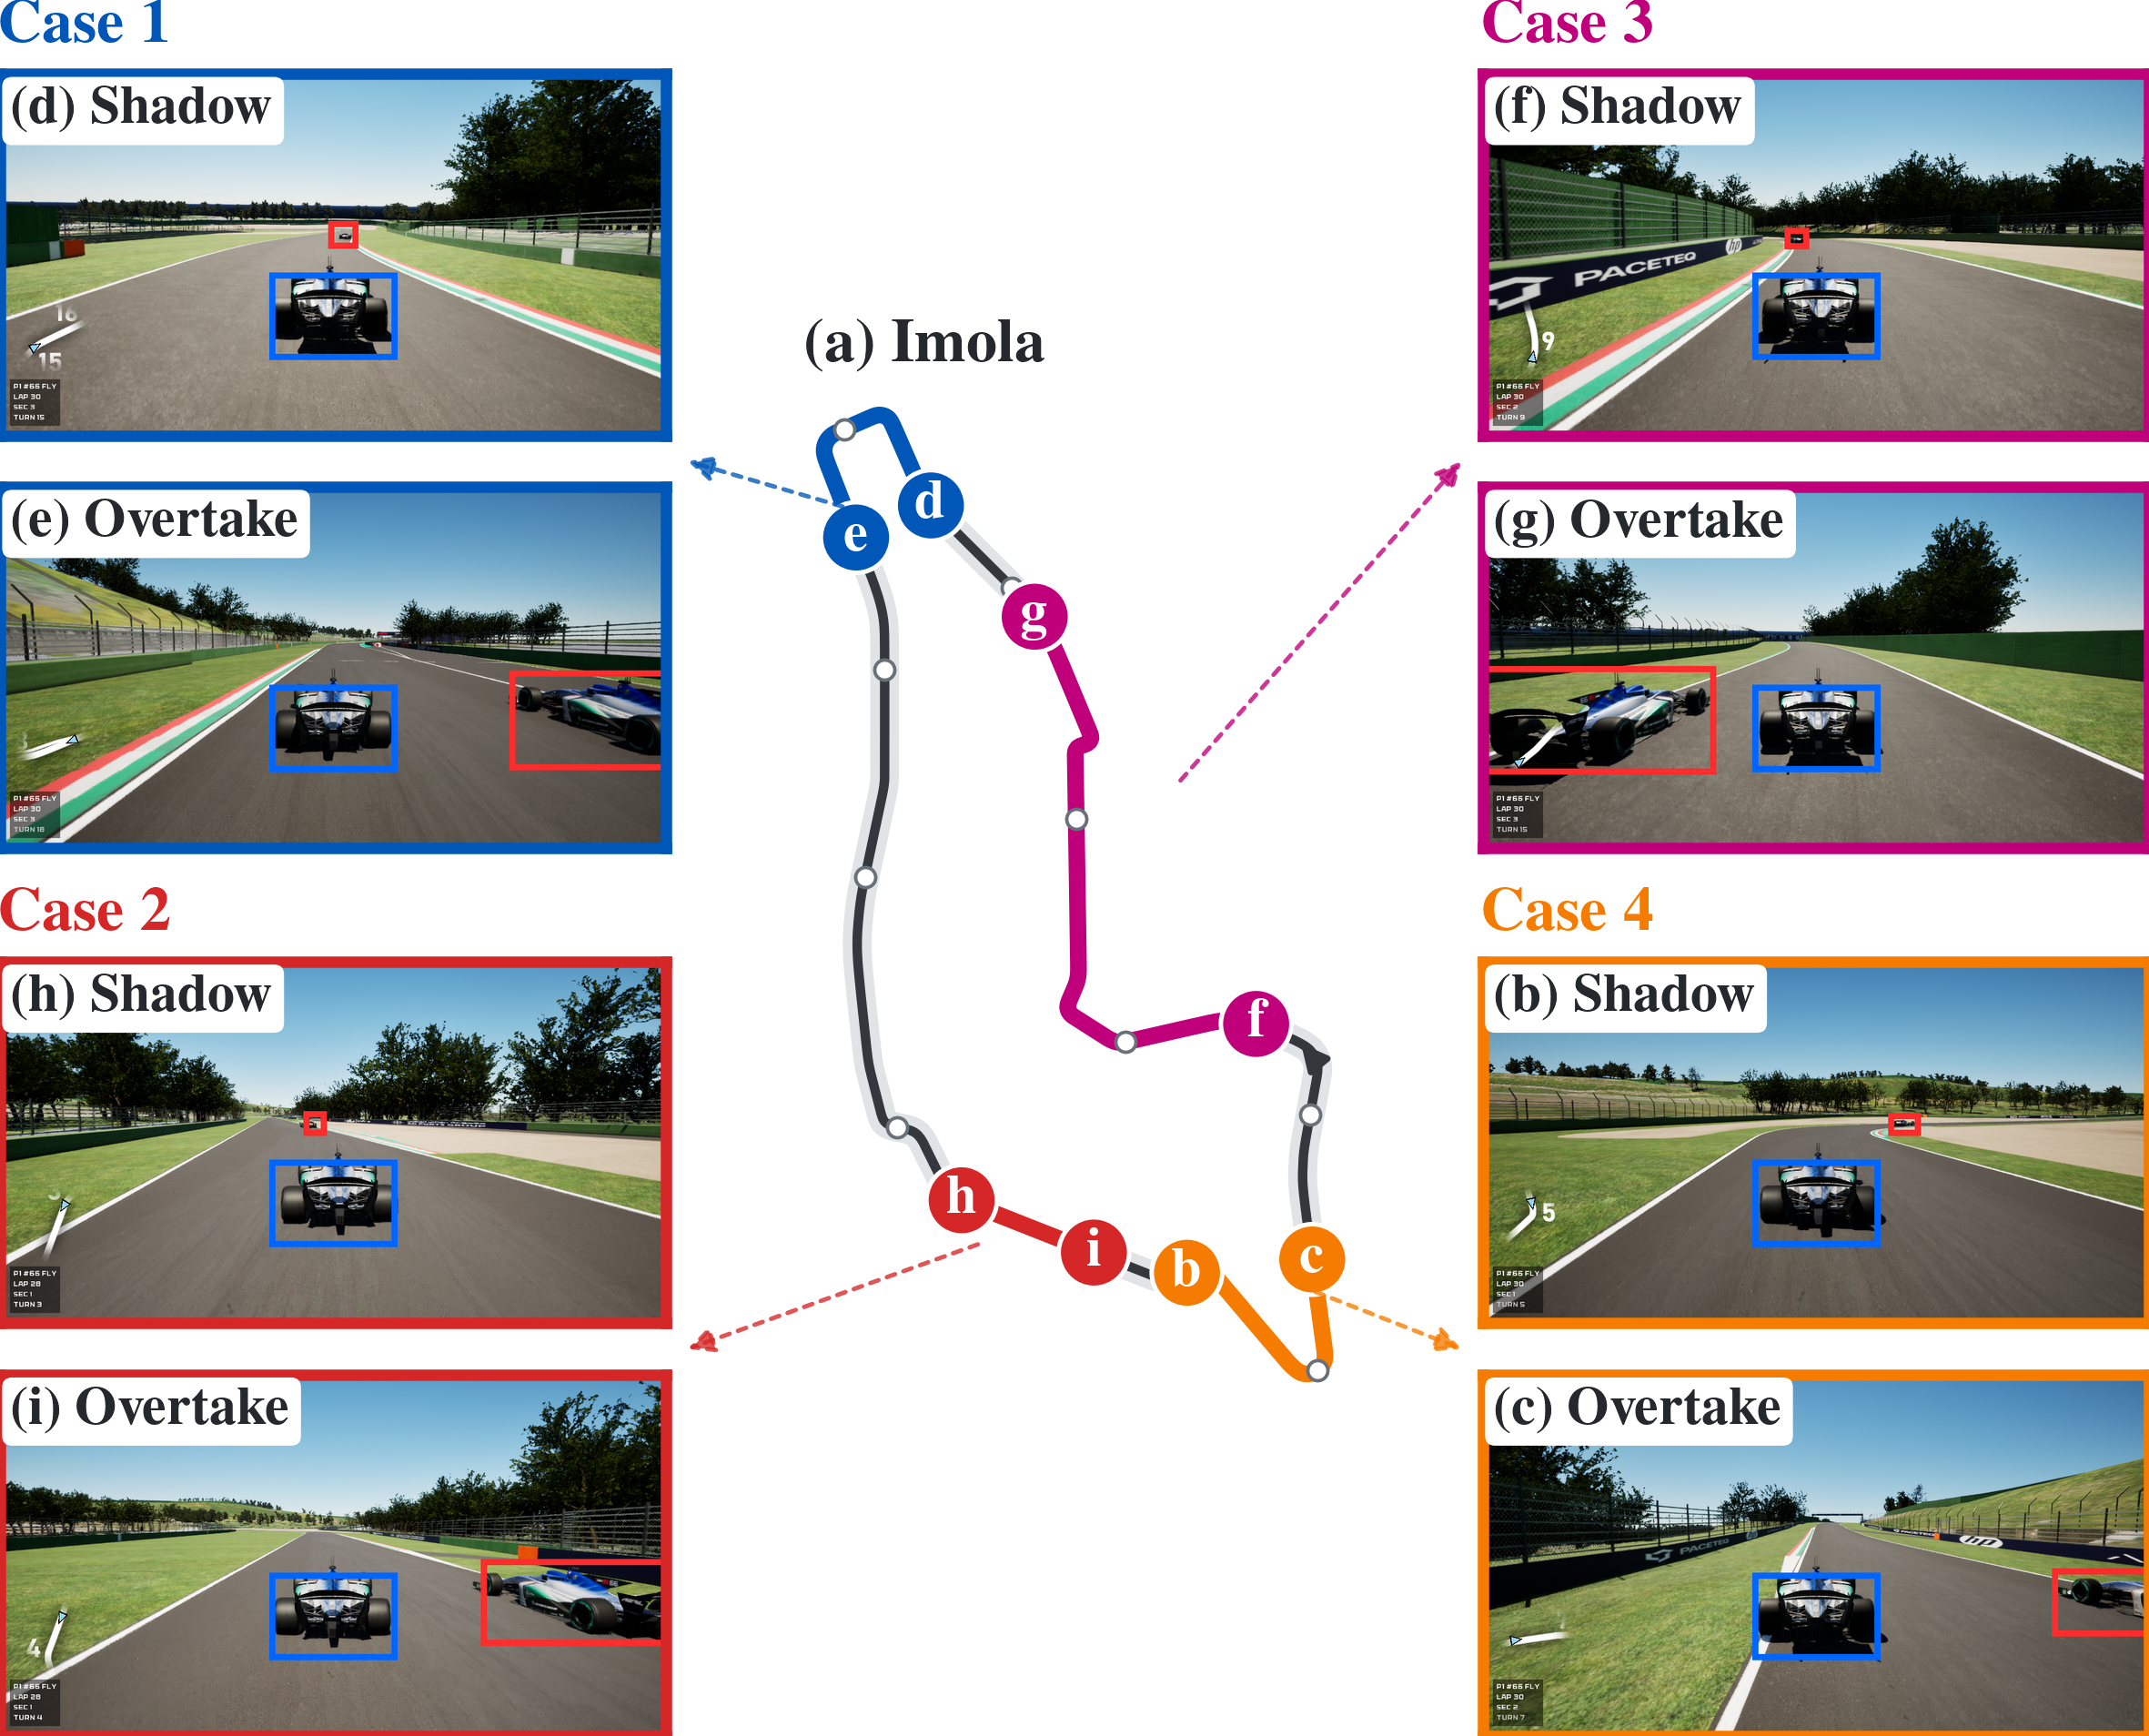
\includegraphics[width=\columnwidth]{track_overview_imola_v006.png}
\caption{未见 Imola 赛道上的典型超车事件。赛道图标出四个事件位置，并在每处给出配对的
\textsc{Shadow} 与 \textsc{Overtake} 模拟器视图。}
\label{fig:imola_overview}
\end{figure}

\begin{figure}[!tbp]
\centering
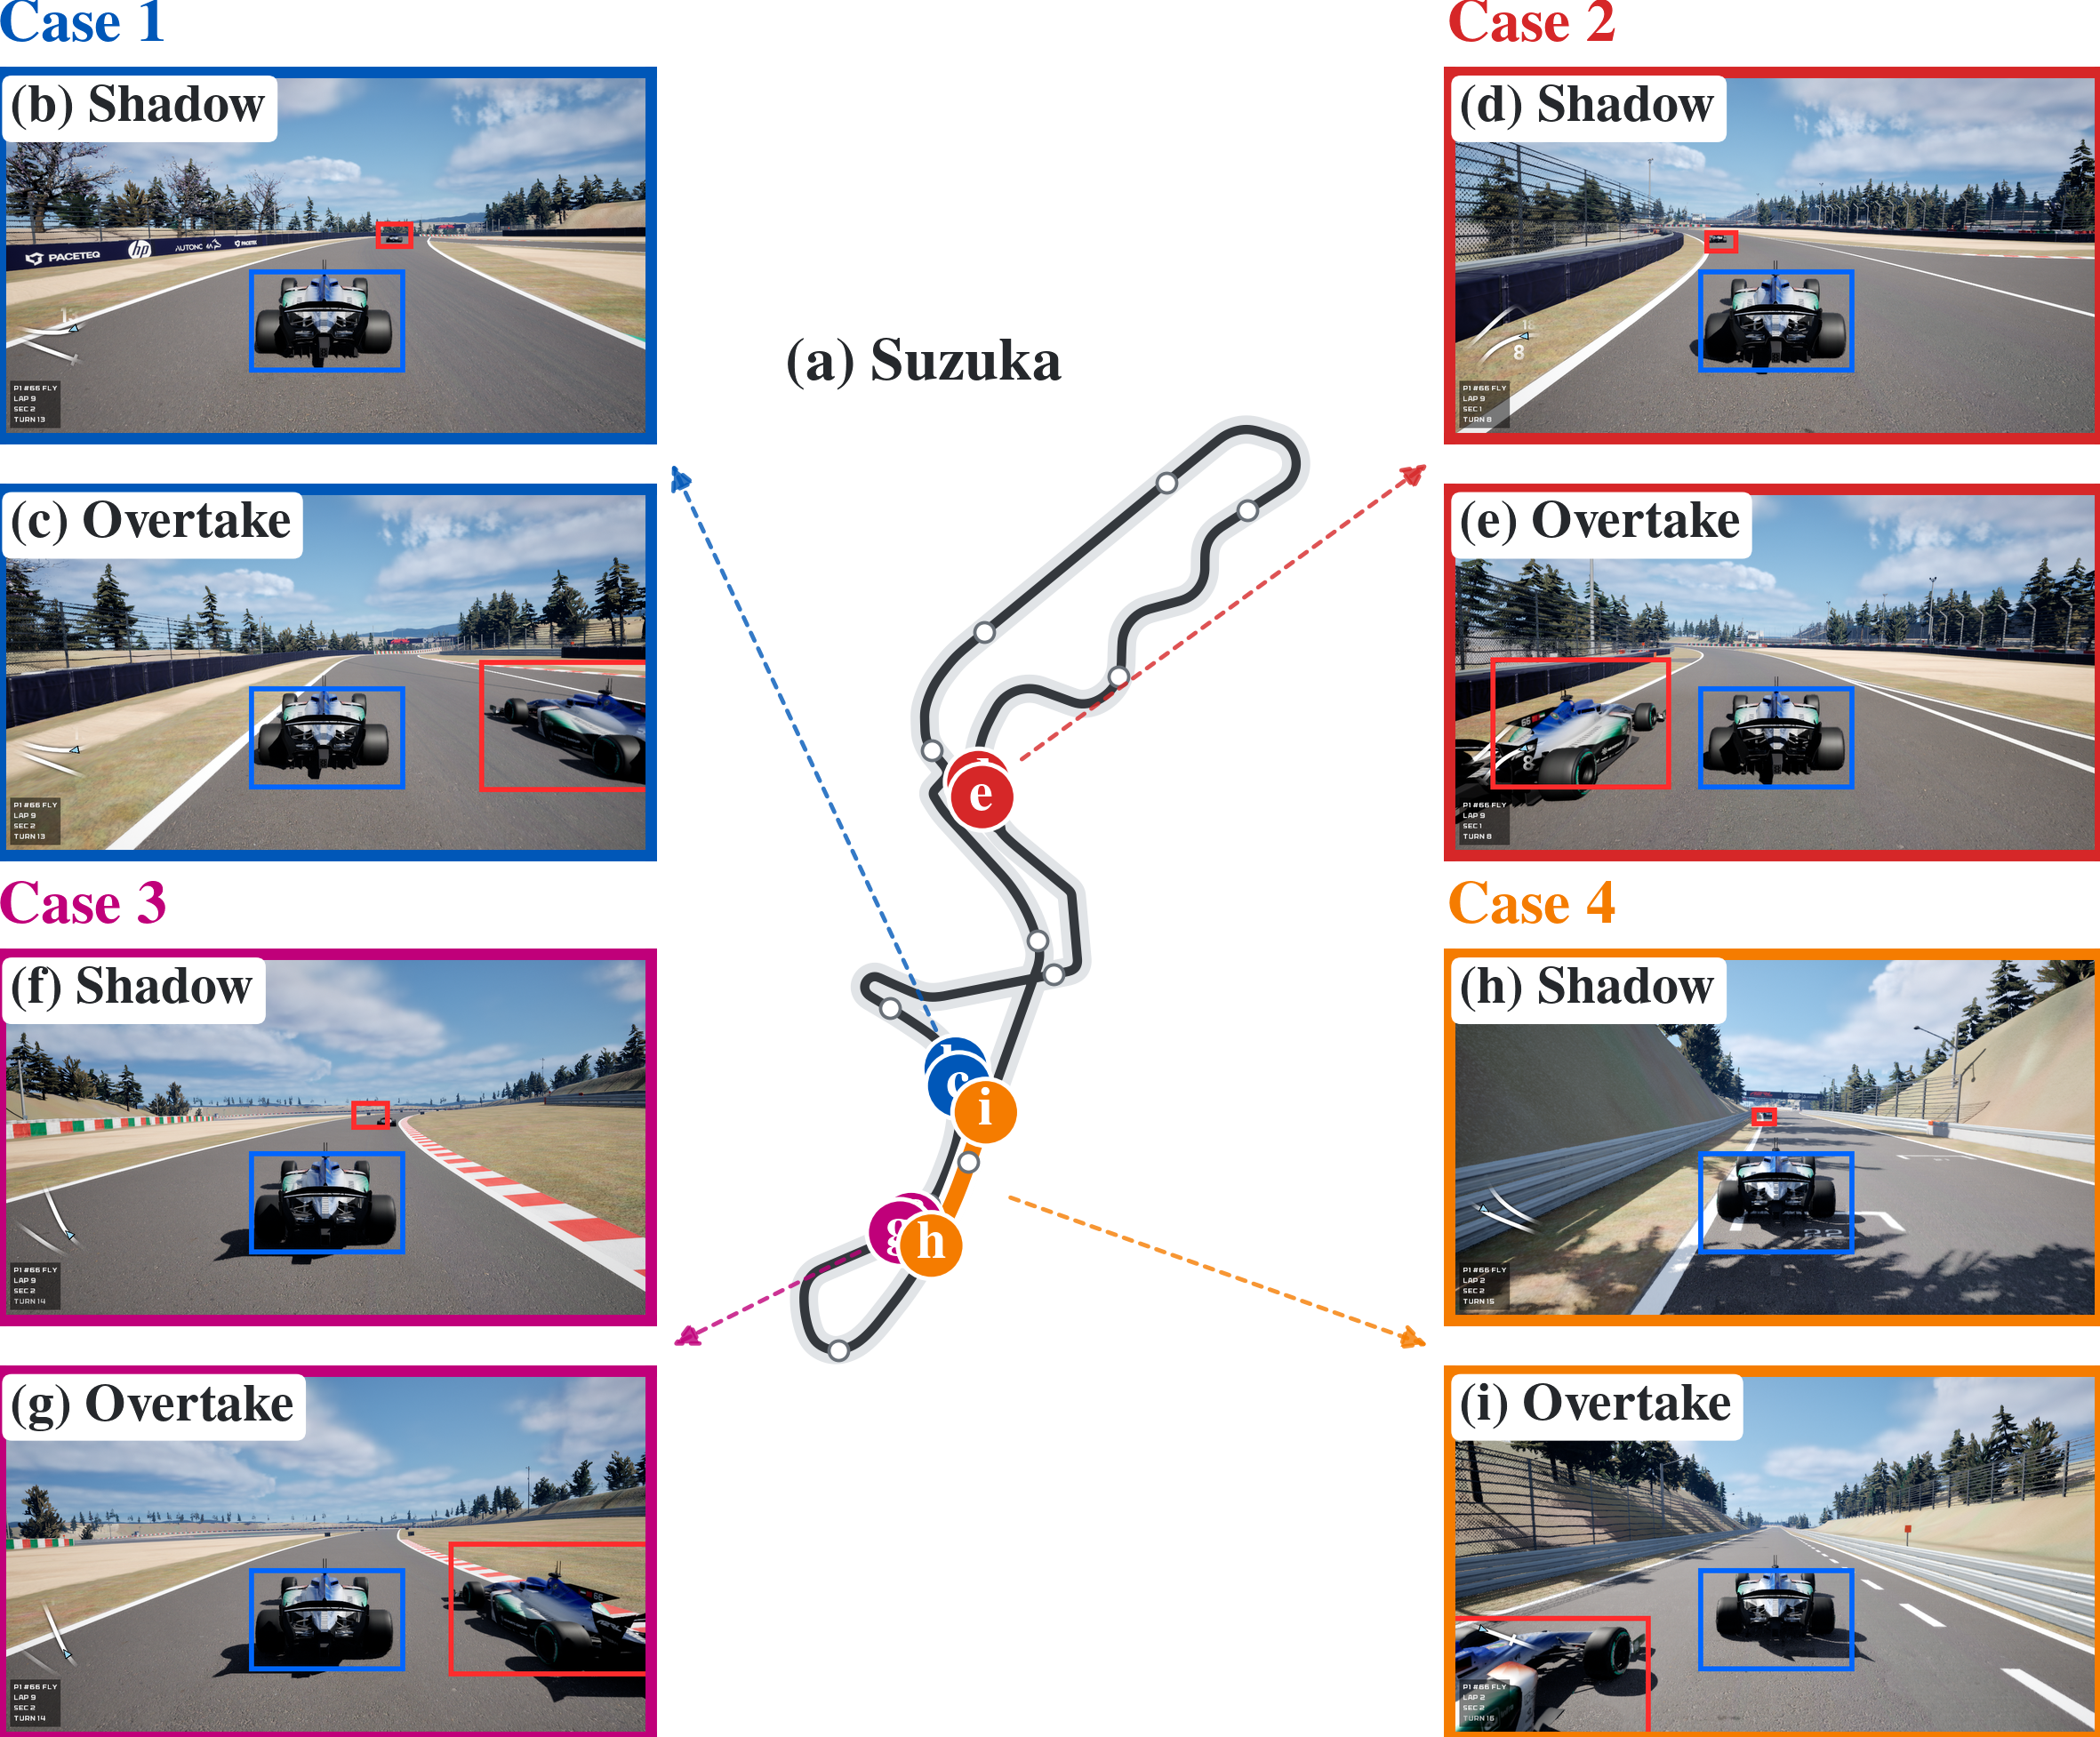
\includegraphics[width=\columnwidth]{track_overview_suzuka_selected_four_v005.png}
\caption{未见 Suzuka 赛道上的典型超车事件。四个赛道位置连接不同局部几何下的接近阶段与
锁定超车阶段。}
\label{fig:suzuka_overview}
\end{figure}

\begin{table}[!tbp]
\centering
\footnotesize
\setlength{\tabcolsep}{3.0pt}
\renewcommand{\arraystretch}{1.05}
\caption{未见赛道上的汇总性能。}
\label{tab:unseen_generalization}
\begin{tabular}{@{}lcc@{}}
\toprule
指标 & Imola & Suzuka \\
\midrule
评估圈数 [次]       & & \\
成功超车 [次] & & \\
OSR [\%；95\%置信区间]             & & \\
TTO [s]                       & & \\
最小间距 [m]               & & \\
平均TTC [s]                  & & \\
接触 [次/$N$]          & & \\
赛道违规 [次/$N$] & & \\
PFR                           & & \\
\bottomrule
\end{tabular}

\vspace{1mm}
\begin{minipage}{0.98\columnwidth}
\scriptsize
\emph{注：}连续指标以均值$\pm$标准差报告；TTO仅对成功超车计算。OSR同时给出双侧精确
二项置信区间；接触和赛道违规以评估圈数内的事件次数报告。
\end{minipage}
\end{table}

在所示八次事件中，战术状态在直道与弯道均由接近演化至锁定超车。表~\ref{tab:unseen_generalization}
中的汇总结果量化了这种跨赛道迁移能力。



% =====================================================================
\section{讨论与局限性}\label{sec:discussion}
% =====================================================================

现有证据支持的是一种架构层面的结论，而非以学习取代基于模型的赛车控制。策略选择何时、
何处锁定机动并发布空间--速度边界，确定性走廊则将该决策显式传递给通用执行器，而不会把
策略噪声传入执行器。由于所有配对方法共享同一执行器，比较与消融将主要增益归因于战术表示：
固定走廊造成最大损失，FSM提供时间持续性，响应集监督改善超车时机与间距。TQC与SAC之间
较小的差异进一步表明，分布式悲观估计是补充因素，而非性能的唯一来源。该定位使本文方法
有别于直接博弈求解器~\cite{liniger2019game,wang2021game,fridovich2020ilqgames}和端到端赛车
策略~\cite{wurman2022gtsophy,fuchs2021superhuman,song2021overtaking}。

参考层轮胎可接受性筛选剔除过大的预瞄需求，包络图则独立评估实际需求。两个详细工况中的全部
记录样本均位于给定包络内，但这一观察并不等同于被控对象层面的约束强制或安全保证。该筛选
也不能解释比较增益，因为所有配对方法均使用同一筛选。目标计算机硬件在环回路保留通信、
求解器回退和执行器分配，因此比离线回放提供更强的执行证据；但其不能替代实车赛道验证，
也没有量化仿真到赛道误差、最坏情况计算时间、感知不确定性以及轮胎和路面条件变化。

因此，当前研究范围限于状态已知的双车硬件在环交互；未见赛道示例提供了定性的几何迁移证据，
但尚不能说明不受限制的泛化能力。后续验证应引入感知相关的走廊不确定性，将响应集教师和
裁剪器扩展至多对手场景，保留逐圈场景、种子、时序和故障标识以开展分层不确定性分析，并在
匹配初始条件下比较硬件在环与EAV24实车赛道执行。这些扩展可在不改变核心可行集接口的前提下
检验迁移边界。

% =====================================================================
\section{结论}\label{sec:conclusion}
% =====================================================================
本文研究了具有战略意义的超车决策与规划器可执行闭环行为之间的衔接问题，提出一种学习持续
战术可行集而非底层控制动作的博弈引导策略。鲁棒Stackelberg响应集教师提供投影后的动作条件
目标并由TQC进行蒸馏；带滞回的状态机和确定性裁剪则将结果转化为供通用执行层使用的时变
Frenet走廊。在双CAN的EAV24硬件在环回路中，方法运行于目标RGS-8805GC计算机，并在1000圈
测试中取得94.7\%的超车成功率，未观察到碰撞或赛道违规。配对基线和消融实验表明，自适应
走廊塑形、博弈引导和持续侧向承诺均对该结果作出贡献。现有证据支持将战术走廊学习作为连接
交互推理与受约束车辆执行的实用接口；轮胎力模型提供辅助性的参考层轮胎可接受性，而非全文
的组织主线。该证据尚不能构成形式化安全保证，也不能说明超出状态已知双车硬件在环交互的
鲁棒性；仍需开展感知相关的多对手与实车赛道试验。

\appendix
\section{算法与评估参数}
\label{app:parameters}
\setcounter{table}{0}

本附录给出复现算法逻辑所需的数值设置与归一化奖励特征。

\begin{table}[!tbp]
\centering
\scriptsize
\setlength{\tabcolsep}{2.0pt}
\renewcommand{\arraystretch}{0.95}
\caption{主要算法与闭环评估设置。}
\label{tab:setup_params}
\begin{tabular}{@{}p{0.21\linewidth}p{0.43\linewidth}p{0.30\linewidth}@{}}
\toprule
组件 & 参数 & 数值 \\
\midrule
车辆几何 & \(m\); \(l_f,l_r\) & \(742\) kg; \(1.75,1.35\) m \\
轮胎曲线 & \(F_{z,0}\); \(C_x,C_y\); \(E_x,E_y\) &
\(2079.72\) N; \(1.6144,1.5998\); \(0,0\) \\
轮胎曲线 & \(\mu_x,\mu_y\); \(s_x,s_y\); \(q_{x,\rm pk},q_{y,\rm pk}\) &
\(2.2345,1.9745\); \(-0.2555,-0.4787\); \(0.1296,0.140\) \\
轮胎包络 & 构造；在线评估 &
准稳态映射~\eqref{eq:tire_accel_envelope}；速度插值 \\
时间尺度 & \(T_{\rm tac}\); \(T_c\); 站点间距 &
\(0.10\) s; \(0.05\) s; \(2\) m \\
响应集教师 & 每侧Sobol候选数；\(\varepsilon_{\rm BR}\);
\(\gamma_g\) & \(64\); \(0.05\); \(0.99\) \\
动作投影 & \(\Delta_g\); \(q_{\rm neu}\) & \(0.5\) m; \(0.25\) \\
FSM & \(N_{\rm post}\); 旧参考上限 &
\(3\)次更新；\(1\)个重新验证周期 \\
TQC & 评论家数；\(N_q\)；保留的\(K\)；\(\gamma\) &
\(2\); \(25\); \(46\); \(0.99\) \\
TQC引导 & \(\lambda_p\); \(\lambda_g\); 先验度量 &
\(1\); \(1\); 动作归一化后的单位度量 \\
走廊 & 预瞄；站点数；\(L_{\min}^{\rm corr}\)；\(\beta\) &
\(300\) m; \(150\); \(3\) m; \(0.2\) \\
Frenet健康检查 & \(\varepsilon_s\); \(\xi_{\max}\); \(\underline v_s\) &
\(0.05\); \(1.30\) rad; \(1\) m s\(^{-1}\) \\
路径健康检查 & 迭代次数；\((\varepsilon_{\rm dyn},\varepsilon_{\rm cor})\) &
\(5\); \((10^{-3},10^{-3}\ {\rm m})\) \\
速度剖面 & \(H_s\); \(V_{\min},v_{x,\max}\); \(\varepsilon_\rho\) &
\(150\); \(15,90\) m s\(^{-1}\); \(10^{-3}\) \\
RC-NMPC & 步数；\(T_c\)；\(\delta_{\max}\)；\(\dot\delta_{\max}\)；
\(\Delta V_{\max}\) &
\(15\); \(0.05\) s; \(0.35\) rad; \(1.0\) rad s\(^{-1}\);
\(0.5\) m s\(^{-1}\) \\
RC-NMPC权重 & \(q_{\Delta\delta},q_c,q_\psi\); \(\bm R_\nu\) &
\(2,20,10\); \(\operatorname{diag}(1,0.5)\) \\
\bottomrule
\end{tabular}
\end{table}

\begin{table}[t]
\centering
\scriptsize
\caption{战术策略边界、奖励权重与训练设置。符号遵循式~\eqref{eq:action_vec}和
式~\eqref{eq:reward_sum}。}
\label{tab:tactical_settings}
\renewcommand{\arraystretch}{0.98}
\begin{tabular}{@{}p{0.29\linewidth}p{0.65\linewidth}@{}}
\toprule
分组 & 设置 \\
\midrule
走廊与速度 & $L^{\rm cap},R^{\rm cap}\in[1.5,6.0]$ m;
$d_{\rm safe}\in[0.2,0.8]$ m;
$V_{\rm cap}^{\rm req}\in[15,90]$ m s$^{-1}$ \\
间距阈值 & $g_{\rm chase}\in[18,24]$ m;
$g_{\rm ot}\in[16,24]$ m; $g_{\rm abort}\in[28,45]$ m \\
偏置、恢复与侧向 & $b_{\rm lat}\in[-1.5,1.5]$ m;
$w_{\rm safe}\in[1,5]$ m; $q_{\rm side}\in[-1,1]$ \\
奖励权重 & \resizebox{\linewidth}{!}{$\begin{gathered}
(w_{\rm ot},w_{\rm ovb},w_{\rm col},w_{\rm lat},w_{\rm crush},w_{\rm app},\\
w_{\rm sm},w_{\rm gs},w_{\rm sbs},w_{\rm wide})\\
=(30,-20,-100,-2,-5,3,-0.1,-0.5,0.5,0.25)
\end{gathered}$} \\
优化 & 学习率 $3\times10^{-4}$；回放容量 $10^5$；
批量大小 $256$；目标更新率 $5\times10^{-3}$ \\
网络 & 独立Actor编码器 $51\!\to\!256\!\to\!256$；共享评论家状态--动作编码器；
两个分位数头；仅训练阶段使用的鲁棒价值头 \\
投影梯度 & 分段 $\Pi_{\mathcal A}$；$\Pi_{\rm tire}$ 前向精确计算；Actor/先验更新采用STE；
Bellman目标停止梯度 \\
软件 & Python \texttt{3.10.0}; SB3 \texttt{2.8.0}; PyTorch
\texttt{2.4.0+cu124}; Gymnasium \texttt{1.2.3} \\
\bottomrule
\end{tabular}
\end{table}

\begingroup
\scriptsize
\setlength{\jot}{0.5pt}
\begin{equation}
\begin{aligned}
\phi_{\rm ot}&=\mathbb{1}[m_t=\textsc{Overtake},
m_{t+1}=\textsc{Raceline},P_t],\\
\phi_{\rm ovb}&=\phi_{\rm ot}\text{（角色互换）},\\
\phi_{\rm col}&=\mathbb{1}[\mathrm{contact}\vee\mathrm{offtrack}
\vee\mathrm{comm\_loss}],\\
\phi_{\rm lat}&=\mathbb{1}[m_t=\textsc{Raceline}]
\operatorname{clip}\!\left(\frac{n_e-n_{\rm rl}}{W_{\rm trk}/2},-1,1\right)^2,\\
\phi_{\rm crush}&=\mathbb{1}[|g_t|<g_{\rm ot}]
\left(\frac{[\rho_{\rm exc}-|\Delta n|]_+}{\rho_{\rm exc}}\right)^2,\\
\phi_{\rm app}&=\mathbb{1}[0<g_t<g_{\rm chase}]
\operatorname{clip}\!\left(\frac{g_{t-1}-g_t}{g_{\rm chase}},0,1\right),\\
\phi_{\rm sm}&=\min\!\left\{1,
\frac{\|\mathsf N_a(\bm a_t^{\rm F})-
\mathsf N_a(\bm a_{t-1}^{\rm F})\|_2^2}{10}\right\},\\
\phi_{\rm gs}&=\min\!\left\{1,\frac{1}{2N_{\rm sta}}
\sum_k\sum_{\pm}\left(\frac{n_{k,t}^{\pm}-n_{k,t-1}^{\pm}}
{W_{{\rm trk},k}}\right)^2\right\},\\
\phi_{\rm sbs}&=\mathbb{1}[|g_t|<g_{\rm ot},
|\Delta n|\ge\rho_{\rm exc}],\\
\phi_{\rm wide}&=\frac{1}{N_{\rm sta}}\sum_k
\operatorname{clip}\!\left(\frac{n_{k,t}^+-n_{k,t}^--L_{\min}^{\rm corr}}
{W_{{\rm trk},k}-L_{\min}^{\rm corr}},0,1\right).
\end{aligned}
\label{eq:reward_features}
\end{equation}
\endgroup



\section*{致谢}
作者感谢阿布扎比自动驾驶赛车联赛提供EAV24仿真与车辆接口环境。


\renewcommand{\bibfont}{\scriptsize}
\begin{thebibliography}{35}

\bibitem{kabzan2020amzracing}
J. Kabzan, M. de la Iglesia Valls, V. J. F. Reijgwart \emph{et al.},
``AMZ Driverless: The full autonomous racing system,''
\emph{Journal of Field Robotics}, vol. 37, no. 7, pp. 1267--1294, 2020.

\bibitem{betz2022survey}
J. Betz, H. Zheng, A. Liniger \emph{et al.},
``Autonomous vehicles on the edge: A survey on autonomous vehicle racing,''
\emph{IEEE Open Journal of Intelligent Transportation Systems}, vol. 3,
pp. 458--488, 2022.

\bibitem{betz2023autonomous}
J. Betz, T. Betz, F. Fent \emph{et al.},
``TUM autonomous motorsport: An autonomous racing software for the Indy
Autonomous Challenge,'' \emph{Journal of Field Robotics}, vol. 40, no. 4,
pp. 783--809, 2023.

\bibitem{jung2023iac}
C. Jung, A. Finazzi, H. Seong \emph{et al.},
``An autonomous system for head-to-head race: Design, implementation and
analysis,'' \emph{IEEE Transactions on Intelligent Transportation Systems},
vol. 24, no. 10, pp. 10470--10486, 2023.

\bibitem{sureshbabu2022autopass}
V. Suresh Babu and M. Behl,
``Threading the needle---Overtaking framework for multi-agent autonomous
racing,'' \emph{SAE International Journal of Connected and Automated
Vehicles}, vol. 5, no. 1, pp. 33--43, 2022,
doi: 10.4271/12-05-01-0004.

\bibitem{kim2023hierarchical}
C. Kim, K. Yi, and J. Park,
``Hierarchical motion planning and control algorithm of autonomous racing
vehicles for overtaking maneuvers,'' in \emph{SAE Technical Paper Series},
2023, Paper 2023-01-0698, doi: 10.4271/2023-01-0698.

\bibitem{ji2023hierarchicalgame}
K. Ji, N. Li, M. Orsag, and K. Han,
``Hierarchical and game-theoretic decision-making for connected and automated
vehicles in overtaking scenarios,'' \emph{Transportation Research Part C:
Emerging Technologies}, vol. 150, art. 104109, 2023,
doi: 10.1016/j.trc.2023.104109.

\bibitem{swain2023cooperative}
S. K. Swain, J. J. Rath, and K. C. Veluvolu,
``Cooperative game theory based robust shared lateral control for driver
vehicle interactions,'' \emph{Control Engineering Practice}, vol. 141,
art. 105678, 2023, doi: 10.1016/j.conengprac.2023.105678.

\bibitem{lopez2022payoff}
V. Lopez, F. Lewis, M. Liu, Y. Wan, S. Nageshrao, and D. Filev,
``Game-theoretic lane-changing decision making and payoff learning for
autonomous vehicles,'' \emph{IEEE Transactions on Vehicular Technology},
vol. 71, no. 4, pp. 3609--3620, 2022,
doi: 10.1109/TVT.2022.3148972.

\bibitem{liniger2019game}
A. Liniger and J. Lygeros,
``A noncooperative game approach to autonomous racing,''
\emph{IEEE Transactions on Control Systems Technology}, vol. 28, no. 3,
pp. 884--897, 2020.

\bibitem{wang2021game}
M. Wang, Z. Wang, J. Talbot, J. C. Gerdes, and M. Schwager,
``Game-theoretic planning for self-driving cars in multivehicle competitive
scenarios,'' \emph{IEEE Transactions on Robotics}, vol. 37, no. 4,
pp. 1313--1325, 2021.

\bibitem{fridovich2020ilqgames}
D. Fridovich-Keil, E. Ratner, L. Peters, A. D. Dragan, and C. J. Tomlin,
``Efficient iterative linear-quadratic approximations for nonlinear
multi-player general-sum differential games,'' in \emph{Proc. IEEE
International Conference on Robotics and Automation (ICRA)}, 2020,
pp. 1475--1481.

\bibitem{jia2023bayesian}
Y. Jia, M. Bhatt, and N. Mehr,
``RAPID: Autonomous multi-agent racing using constrained potential dynamic
games,'' in \emph{Proc. European Control Conference (ECC)}, 2023, pp. 1--8.

\bibitem{kalaria2025alpha}
D. Kalaria, C. Maheshwari, and S. Sastry,
``$\alpha$-RACER: Real-time algorithm for game-theoretic motion planning and
control in autonomous racing using $\alpha$-potential function,'' in
\emph{Proc. Learning for Dynamics and Control Conference}, PMLR, vol. 283,
pp. 1--18, 2025.

\bibitem{wurman2022gtsophy}
P. R. Wurman, S. Barrett, K. Kawamoto \emph{et al.},
``Outracing champion Gran Turismo drivers with deep reinforcement learning,''
\emph{Nature}, vol. 602, no. 7896, pp. 223--228, 2022.

\bibitem{yuan2022drlgame}
M. Yuan, J. Shan, and K. Mi,
``Deep reinforcement learning based game-theoretic decision-making for
autonomous vehicles,'' \emph{IEEE Robotics and Automation Letters}, vol. 7,
no. 2, pp. 818--825, 2022, doi: 10.1109/LRA.2021.3134249.

\bibitem{fuchs2021superhuman}
F. Fuchs, Y. Song, E. Kaufmann, D. Scaramuzza, and P. D\"urr,
``Super-human performance in Gran Turismo Sport using deep reinforcement
learning,'' \emph{IEEE Robotics and Automation Letters}, vol. 6, no. 3,
pp. 4257--4264, 2021.

\bibitem{evans2023trajectory}
B. D. Evans, H. A. Engelbrecht, and H. W. Jordaan,
``High-speed autonomous racing using trajectory-aided deep reinforcement
learning,'' \emph{IEEE Robotics and Automation Letters}, vol. 8, no. 9,
pp. 5353--5359, 2023, doi: 10.1109/LRA.2023.3295252.

\bibitem{hell2024lidar}
M. Hell, G. Hajgat\'o, \'A. Bog\'ar-N\'emeth \emph{et al.},
``A LiDAR-based approach to autonomous racing with model-free reinforcement
learning,'' in \emph{Proc. IEEE Intelligent Vehicles Symposium (IV)}, 2024,
pp. 258--263, doi: 10.1109/IV55156.2024.10588613.

\bibitem{song2021overtaking}
Y. Song, H. Lin, E. Kaufmann, P. D\"urr, and D. Scaramuzza,
``Autonomous overtaking in Gran Turismo Sport using curriculum reinforcement
learning,'' in \emph{Proc. IEEE International Conference on Robotics and
Automation (ICRA)}, 2021, pp. 9403--9409.

\bibitem{lin2023limit}
H. Lin, Y. Song, and D. Scaramuzza,
``Reaching the limit in autonomous racing: Optimal control versus
reinforcement learning,'' \emph{Science Robotics}, vol. 8, no. 82,
art. eadg1462, 2023.

\bibitem{hu2023dynamicgraph}
X. Hu, Y. Liu, B. Tang, J. Yan, and L. Chen,
``Learning dynamic graph for overtaking strategy in autonomous driving,''
\emph{IEEE Transactions on Intelligent Transportation Systems}, vol. 24,
no. 11, pp. 11921--11933, 2023, doi: 10.1109/TITS.2023.3287223.

\bibitem{baumann2025predictive}
N. Baumann, E. Ghignone, C. Hu, B. Hildisch, T. H\"ammerle,
A. Bettoni, A. Carron, L. Xie, and M. Magno,
``Predictive Spliner: Data-driven overtaking in autonomous racing using
opponent trajectory prediction,'' \emph{IEEE Robotics and Automation
Letters}, vol. 10, no. 2, pp. 1816--1823, 2025,
doi: 10.1109/LRA.2024.3519878.

\bibitem{han2024marl}
S. Han, S. Zhou, J. Wang, L. Pepin, C. Ding, J. Fu, and F. Miao,
``A multi-agent reinforcement learning approach for safe and efficient
behavior planning of connected autonomous vehicles,''
\emph{IEEE Transactions on Intelligent Transportation Systems}, vol. 25,
no. 5, pp. 3654--3670, 2024, doi: 10.1109/TITS.2023.3336670.

\bibitem{liu2023proactive}
Y. Liu, A. Zhou, Y. Wang, and S. Peeta,
``Proactive longitudinal control to preclude disruptive lane changes of
human-driven vehicles in mixed-flow traffic,''
\emph{Control Engineering Practice}, vol. 136, art. 105522, 2023,
doi: 10.1016/j.conengprac.2023.105522.

\bibitem{guo2025rlhf}
H. Guo, R. Khaire, and J. Zhao,
``Reinforcement learning from human feedback with fast--slow updates for
stable driving strategies,'' \emph{Control Engineering Practice}, vol. 165,
art. 106549, 2025, doi: 10.1016/j.conengprac.2025.106549.

\bibitem{muzahid2025merging}
A. J. M. Muzahid, Y. Shi, Z. Wang, A. Zhou, A. Cook, C. R. Wang, and Z. Wang,
``Optimizing on-ramp merging for connected and automated vehicles: A
hierarchical approach using deep reinforcement learning and optimal control,''
\emph{Control Engineering Practice}, vol. 165, art. 106614, 2025,
doi: 10.1016/j.conengprac.2025.106614.

\bibitem{thakkar2024hierarchical}
R. S. Thakkar, A. S. Samyal, D. Fridovich-Keil, Z. Xu, and U. Topcu,
``Hierarchical control for head-to-head autonomous racing,''
\emph{Field Robotics}, vol. 4, no. 1, pp. 46--69, 2024,
doi: 10.55417/FR.2024002.

\bibitem{hoffmann2026a2rl}
S. Hoffmann, S. Sagmeister, T. Betz \emph{et al.},
``Head-to-head autonomous racing at the limits of handling in the A2RL
challenge,'' arXiv preprint arXiv:2602.08571, 2026.

\bibitem{kuznetsov2020tqc}
A. Kuznetsov, P. Shvechikov, A. Grishin, and D. Vetrov,
``Controlling overestimation bias with truncated mixture of continuous
distributional quantile critics,'' in \emph{Proc. 37th International
Conference on Machine Learning}, PMLR, vol. 119, pp. 5556--5566, 2020.

\bibitem{yang2026corridor}
C. Yang, H. Liu, Z. Li, X. Zhang, X. Zhao, and B. Wang,
``Hierarchical cooperative planning incorporating MARL guidance and
interactive spatio-temporal corridor constraints,''
\emph{Control Engineering Practice}, vol. 175, art. 107120, 2026,
doi: 10.1016/j.conengprac.2026.107120.

\bibitem{toschi2025modular}
A. Toschi, F. Prignoli, and M. Bertogna,
``Modular decision-making and drivable areas for multi-agent autonomous
racing,'' in \emph{Proc. IEEE/RSJ International Conference on Intelligent
Robots and Systems (IROS)}, 2025, pp. 12435--12441,
doi: 10.1109/IROS60139.2025.11246897.

\bibitem{veneri2020free}
M. Veneri and M. Massaro,
``A free-trajectory quasi-steady-state optimal-control method for minimum
lap-time of race vehicles,''
\emph{Vehicle System Dynamics}, vol. 58, no. 6, pp. 933--954, 2020,
doi: 10.1080/00423114.2019.1608364.

\bibitem{a2rl2024}
Abu Dhabi Autonomous Racing League (A2RL),
``Autonomous car race 2024,'' 2024. [Online]. Available:
\url{https://a2rl.io/autonomous-car-race/car-race-2024}
(accessed 18 August 2026).

\bibitem{neousysrgs}
Neousys Technology Inc., ``RGS-8805GC AMD EPYC 7003 series rugged HPC server:
Product datasheet,'' 2023. [Online]. Available:
\url{https://www.neousys-tech.com/product/product-lines/rugged-industrial-hpc-server/rgs-8805gc}.

\end{thebibliography}



\end{document}
